\documentclass[12pt,a4paper]{article}

\usepackage[margin=2.5cm,headheight=14pt]{geometry}
\usepackage{amsmath,amssymb,amsfonts}
\usepackage{graphicx}
\usepackage[round]{natbib}
\usepackage{booktabs}
\usepackage{float}
\usepackage{caption}
\usepackage{hyperref}
\usepackage{xcolor}
\usepackage{enumitem}
\usepackage{setspace}
\usepackage{fancyhdr}
\usepackage{amsthm}

\newtheorem{proposition}{Proposition}

\definecolor{primary}{RGB}{30,60,114}
\definecolor{secondary}{RGB}{100,100,100}

\pagestyle{fancy}
\fancyhf{}
\fancyhead[L]{\small\color{secondary}Zhang (2026): FOMC Communication and Bank Stress}
\fancyfoot[C]{\thepage}

\onehalfspacing
\setlength{\parindent}{2em}
\setlength{\parskip}{0.5em}

\captionsetup{font=small,labelfont=bf}
\captionsetup[table]{position=above}
\captionsetup[figure]{position=below}

\title{\color{primary}\textbf{FOMC Communication and Bank Stress:\\ Information Hierarchy, Signal Divergence, and the Pre/Post-2008 Regime Shift}}
\author{Eileen Zhang}
\date{June 2026}

\begin{document}
\maketitle

\begin{abstract}
We test whether FOMC statement language functions as a real-time indicator of bank stress, using 216 FOMC meetings (1994--2025) matched to daily returns of 24 US DFAST banks and 11 Japanese megabanks and regional banks. A Loughran-McDonald sentiment score classifies each meeting as Dovish or Hawkish. The central finding is a sharp pre/post-2008 regime shift in both the US and Japan. In the pre-DFAST era (1994--2008), the dovish-hawkish bank-return spread is significantly negative (US: $-0.89$pp, $t = -2.13$; Japan: $-1.40$pp, $t = -2.24$), consistent with a distress-signal interpretation. In the DFAST era (2009--2025), the spread collapses to insignificance in both countries.

We further decompose the cross-sectional transmission into four independent channels using FR Y-9C balance-sheet data for 14 US BHCs. (1) NIM compression channel: during ZLB periods, high-NIM banks benefit more from dovish FOMC (Dovish\,$\times$\,ZLB\,$\times$\,NIM = +0.68, t = 3.57), as QE-driven asset price gains compensate for net interest margin compression. (2) CRE sensitivity channel: high-CRE banks benefit more from dovish FOMC during ZLB (Dovish\,$\times$\,ZLB\,$\times$\,CRE = +0.25, t = 2.47), reflecting CRE loan valuation gains. (3) HTM unrealized loss channel: during the 2022–23 rapid rate hikes, high-HTM banks suffer significantly larger losses (FastHike\,$\times$\,HTM = -0.09, t = -7.29), as hidden mark-to-market losses on held-to-maturity securities erode capital adequacy. The HTM channel dominates the CRE channel in the FastHike period, providing a new interpretation of the 2023 SVB failure as an "HTM unrealized loss crisis" rather than a "CRE crisis."  (4) Information hierarchy channel: we construct a three-document FOMC corpus (Statement, Minutes, Transcript) and classify each using both LM\% and LLM. Statement-Minutes agreement is only 30.7\%. When Statement and Minutes diverge, bank CAR is significantly worse (-0.247pp vs +0.174pp, spread = 0.421pp). The effect is US-specific, amplified in the inflation era (r = -0.336, p = 0.034), and strongest when the LLM is highly confident yet wrong (r = -0.260, p = 0.029). Transcripts validate Minutes over Statements. Adding Minutes information increases R-squared from 0.07\% to 2.87\%. The 2013 Taper Tantrum exhibits the highest stance distance (z-score = 4.58). A within-bank quasi-experiment isolates the causal effect of accounting classification: the same bank holds both HTM and AFS securities with identical cash flows, differing only in accounting treatment. The $\Delta$ test yields $-0.054$ (t = $-6.93$), confirming that non-mark-to-market accounting is the causal mechanism. The NIM channel's microfoundation is validated through the rebalancing channel: Dovish\,$\times$\,ZLB\,$\times$\,NIM\,$\times$\,TradingRatio = $+0.0048$ (t = $2.79$). A Kuttner surprise robustness check decomposes the transmission into two complementary mechanisms: the \textit{interest rate mechanism} (HTM and NIM channels are driven by rate surprises) and the \textit{information mechanism} (LM\% captures forward guidance beyond the rate decision). The cross-sectional-to-aggregate mapping reveals that the system-level cumulative CAR under the FastHike scenario is $-0.88$\%, with SVB's extreme HTM ratio explaining 76\% of its predicted loss. All four channels are robust to excluding the COVID ZLB period and to GSIB vs. regional bank subsample splits.
\end{abstract}

\noindent\textbf{Keywords:} FOMC Communication; Bank Stress; Regime Shift; Information Hierarchy; Signal Divergence; HTM Unrealized Losses; NIM Compression

\noindent\textbf{JEL Codes:} E44, E52, E58, G01, G14, G21, G28, C55

\newpage

\section{Introduction}

When Silicon Valley Bank collapsed on March 10, 2023, its held-to-maturity (HTM) securities portfolio carried \$15.2 billion in unrealized losses---26\% of total assets---that had accumulated during the Federal Reserve's fastest rate-hiking cycle in four decades. Yet the Fed's own stress test (DFAST/CCAR) had never flagged this risk. The DFAST severely adverse scenario tests credit risk and interest rate risk in the banking book, but does not model the information asymmetry created by HTM accounting: when rates rise rapidly, HTM securities generate hidden capital erosion that is invisible to market participants until a liquidity event forces recognition. This paper asks a broader question: does the language of FOMC statements---publicly available in real time---contain information about the cross-section of bank stress that stress tests miss?

We classify each of 216 FOMC meetings (1994--2025) as Dovish or Hawkish using the Loughran-McDonald sentiment score (\citet{Loughran2011}), and measure bank-level cumulative abnormal returns (CARs) around each meeting. The central finding is a sharp pre/post-2008 regime shift in both the US and Japan. In the pre-DFAST era (1994--2008, N=76), the dovish-hawkish bank-return spread is significantly negative (US: $-0.89$pp; Japan: $-1.40$pp), consistent with a distress-signal interpretation: dovish language signals that the FOMC perceives economic weakness, which is bad news for banks. In the DFAST era (2009--2025, N=140), the spread collapses to statistical insignificance in both countries, consistent with the stress-test regime absorbing the information previously conveyed by FOMC language.

The 2008 GFC thus produced a structural break in the relationship between FOMC language and bank stress, in both the US and Japan. Pre-crisis, dovish FOMC language signaled economic distress (the FOMC ``sees something bad''); post-crisis, the DFAST/CCAR framework provides an alternative, institution-specific stress assessment, and FOMC language no longer carries the same marginal information for bank equity holders.

Balance-sheet data validates the cross-sectional interpretation across 20 US BHCs using a combination of FR Y-9C (14 BHCs) and FFIEC 031 Call Reports (6 additional BHCs). High-CRE US banks show a $-0.40$pp dovish-hawkish spread vs.\ $-0.22$pp for low-CRE banks. Capital-building banks (positive tier1\_yoy\_pct) show a $-0.48$pp spread vs.\ $-0.20$pp for capital-depleting banks.

We decompose the cross-sectional transmission into four independent channels using panel regressions with bank and time fixed effects. The NIM compression channel captures the fact that during ZLB periods, dovish FOMC signals QE-driven asset price gains that compensate high-NIM banks for margin compression (Dovish\,$\times$\,ZLB\,$\times$\,NIM = +0.68, $p < 0.001$). The CRE sensitivity channel captures CRE loan valuation gains from low interest rates (Dovish\,$\times$\,ZLB\,$\times$\,CRE = +0.25, $p = 0.013$). The HTM unrealized loss channel captures the asymmetric risk of held-to-maturity securities during rapid rate hikes: high-HTM banks suffer significantly larger losses (FastHike\,$\times$\,HTM = $-0.09$, $p < 0.001$), as hidden mark-to-market losses erode capital adequacy. Critically, the HTM channel dominates the CRE channel in the FastHike period, providing a new interpretation of the 2023 SVB failure as an ``HTM unrealized loss crisis'' rather than a ``CRE crisis.''

Three additional analyses strengthen these findings. First, a within-bank quasi-experiment isolates the causal effect of accounting classification: the same bank holds both HTM and AFS securities with identical cash flows, differing only in accounting treatment. The $\Delta$ test yields $-0.054$ (t = $-6.93$), confirming that non-mark-to-market accounting is the causal mechanism. Second, the NIM channel's microfoundation is validated through the rebalancing channel: Dovish\,$\times$\,ZLB\,$\times$\,NIM\,$\times$\,TradingRatio = $+0.0048$ (t = $2.79$) confirms that trading income compensates for NIM compression during ZLB periods. Third, a Kuttner surprise robustness check decomposes the transmission into two complementary mechanisms: the \textit{interest rate mechanism} (HTM and NIM channels are driven by rate surprises) and the \textit{information mechanism} (LM\% captures forward guidance beyond the rate decision).

The cross-sectional-to-aggregate mapping translates these bank-level effects into system-level risk measures. Under the FastHike scenario, the system-level cumulative CAR is $-0.88$\%, with the top three banks contributing 47\% of the impact. The SVB counterfactual analysis reveals that SVB's extreme HTM ratio explains 76\% of its predicted loss, providing a quantitative validation of the HTM channel's macro significance.

Section~\ref{sec:theory} develops the theoretical framework. Section~\ref{sec:data} describes the data and methodology, including the new three-document FOMC corpus. Section~\ref{sec:results} reports the US results and the channel decomposition. Section~\ref{sec:japan} reports the Japan results. Section~\ref{sec:comparison} compares US and Japan. Section~\ref{sec:aggregate} presents the cross-sectional-to-aggregate mapping. Section~\ref{sec:reverse} presents the reverse stress test application. Section~\ref{sec:hierarchy} presents the information hierarchy and signal divergence analysis. Section~\ref{sec:discussion} discusses implications. Section~\ref{sec:conclusion} concludes.

\section{Theoretical Framework}\label{sec:theory}

\subsection{Setup}

We develop a stylized model to organize our empirical analysis. Consider a bank $i$ with equity value $E_i$ that holds three asset classes: loans (proportional share $\ell_i$), HTM securities (share $h_i$), and AFS/trading securities (share $a_i = 1 - \ell_i - h_i$). The bank funds these assets with deposits and equity. An FOMC meeting produces a monetary shock $s_t$ (positive = tightening) and a semantic signal $\sigma_t$ (LM\% sentiment).

The bank's CAR around the FOMC meeting is:
\begin{equation}\label{eq:car}
\text{CAR}_{i,t} = \underbrace{\beta_0 s_t}_{\text{rate channel}} + \underbrace{\gamma_0 \sigma_t}_{\text{information channel}} + \underbrace{\beta_1 h_i \cdot s_t \cdot \mathbb{1}[\text{FastHike}]}_{\text{HTM channel}} + \underbrace{\gamma_1 n_i \cdot \sigma_t \cdot \mathbb{1}[\text{ZLB}]}_{\text{NIM channel}} + \varepsilon_{i,t}
\end{equation}
where $n_i$ is the bank's NIM and $\mathbb{1}[\cdot]$ are regime indicators. The key feature is that the HTM channel operates through the \textit{rate} shock $s_t$ while the NIM channel operates through the \textit{semantic} signal $\sigma_t$, reflecting their different economic mechanisms.

\subsection{Propositions and Testable Predictions}

\begin{proposition}[HTM Channel]\label{prop:htm}
During rapid rate hikes ($\mathbb{1}[\text{FastHike}] = 1$), banks with higher HTM ratios experience larger CAR declines: $\beta_1 < 0$. This effect is specific to HTM securities and does not apply to AFS securities, because AFS mark-to-market losses are already reflected in equity via accumulated other comprehensive income (AOCI), while HTM losses remain hidden until realized.
\end{proposition}

\noindent\textit{Testable implication}: FastHike\,$\times$\,HTM $< 0$ while FastHike\,$\times$\,AFS $\approx 0$. The $\Delta$ test (HTM coefficient minus AFS coefficient) isolates the causal effect of accounting classification, holding cash-flow fundamentals constant within the same bank.

\begin{proposition}[NIM Rebalancing Channel]\label{prop:nim}
During ZLB periods ($\mathbb{1}[\text{ZLB}] = 1$), the NIM channel operates through portfolio rebalancing: $\gamma_1 > 0$. Dovish FOMC language signals continued QE, which raises asset prices. High-NIM banks---effectively ``bond-like'' assets---benefit from rebalancing flows, but only if they have trading capacity to capture the gains. Formally:
\begin{equation}\label{eq:rebalancing}
\frac{\partial \text{CAR}_{i,t}}{\partial \sigma_t \cdot \mathbb{1}[\text{ZLB}]} = \gamma_1 n_i + \gamma_2 n_i \cdot \tau_i
\end{equation}
where $\tau_i$ is the trading ratio and $\gamma_2 > 0$ is the rebalancing compensation effect.
\end{proposition}

\noindent\textit{Testable implication}: Dovish\,$\times$\,ZLB\,$\times$\,NIM\,$\times$\,TradingRatio $> 0$ (rebalancing compensation). Conversely, Dovish\,$\times$\,ZLB\,$\times$\,NIM\,$\times$\,DepositRatio $< 0$ (deposit trap: sticky deposit betas prevent NIM recovery).

\begin{proposition}[Regime Shift]\label{prop:regime}
The aggregate sensitivity of bank returns to FOMC language declines after the introduction of stress testing: $|\partial \bar{\text{CAR}}_t / \partial \sigma_t|$ is smaller in the DFAST era than in the pre-DFAST era. This occurs because stress tests provide an alternative, institution-specific assessment that substitutes for the information previously conveyed by FOMC language.
\end{proposition}

\noindent\textit{Testable implication}: The dovish-hawkish bank-return spread is significantly negative in the pre-DFAST era and statistically insignificant in the DFAST era, in both the US and Japan.

\begin{proposition}[Uncertainty Channel]\label{prop:uncertainty}
When word-count sentiment ($\sigma_t^{\text{LM}}$) and LLM semantic classification ($\sigma_t^{\text{LLM}}$) disagree---measured by stance distance $d_t = |\sigma_t^{\text{LM}} - \sigma_t^{\text{LLM}}|$---the resulting uncertainty amplifies bank stress: $\partial \text{CAR}_{i,t} / \partial d_t < 0$. The effect is stronger during ZLB periods, where policy ambiguity is most costly.
\end{proposition}

\noindent\textit{Testable implication}: Stance distance significantly predicts worse bank CAR and higher cross-sectional dispersion, with ZLB amplification.

\subsection{From Cross-Section to Aggregate}

Propositions~\ref{prop:htm} and~\ref{prop:nim} characterize the cross-sectional sensitivity of bank CARs to FOMC shocks. To translate these into system-level risk measures, we aggregate using asset weights:
\begin{equation}\label{eq:aggregate}
\text{System CAR}_t = \sum_{i=1}^{N} w_i \cdot \widehat{\text{CAR}}_{i,t}, \quad w_i = \frac{\text{Assets}_i}{\sum_j \text{Assets}_j}
\end{equation}
This mapping requires the assumption that the cross-sectional elasticities estimated from our panel regressions apply at the system level---that is, the marginal effect of an FOMC shock on bank $i$'s CAR does not depend on the composition of the banking system. We discuss this assumption and its limitations in Section~\ref{sec:aggregate}.

\subsection{Identification}

Our identification strategy exploits three sources of variation. First, the \textit{within-bank} comparison of HTM vs AFS securities (Proposition~\ref{prop:htm}) holds bank-level fundamentals constant, isolating the causal effect of accounting classification. This is analogous to the dual-share identification in \citet{LuWu2024}, who exploit within-firm variation in rebalancer ownership across share classes with identical cash flows. Second, the \textit{regime shift} (Proposition~\ref{prop:regime}) provides a natural experiment: the introduction of DFAST/CCAR in 2009 exogenously changed the information environment. Third, the \textit{Kuttner surprise} decomposition separates the rate channel ($s_t$) from the information channel ($\sigma_t$), confirming that the two mechanisms are complementary rather than substitutive.

We acknowledge two limitations. First, the HTM ratio may be endogenous: banks that choose to classify securities as HTM may differ systematically from those that do not. We address this by noting that (a) the within-bank comparison controls for all time-invariant bank characteristics, and (b) the placebo test using non-FastHike meetings shows no HTM-AFS asymmetry, ruling out time-invariant selection. However, time-varying selection---for example, banks shifting securities into HTM in anticipation of rate hikes---remains a concern. We discuss this further in Section~\ref{sec:discussion}. Second, our Kuttner surprise measure is constructed from daily FFR changes rather than Fed Funds Futures, and may understate the true surprise component. Future work with CME futures data could refine this decomposition.

\section{Data and Methodology}\label{sec:data}

\subsection{FOMC Statement Corpus and LM Sentiment}

We collect 216 FOMC meeting dates from May 1994 through December 2025, with the LM\% sentiment score for each meeting computed using the Loughran-McDonald financial lexicon (\citet{Loughran2011}). Median LM\% in the sample is 3.3\%; meetings below median are classified as Dovish, above as Hawkish.

\subsection{Three-Document FOMC Corpus}

We extend the single-document analysis to a three-document information hierarchy. For each FOMC meeting, we collect: (1) the FOMC Statement ($\sim$800 words, released immediately after the meeting), (2) the FOMC Minutes ($\sim$6,400 words, released approximately three weeks later), and (3) the FOMC Transcript ($\sim$30,000 words, released with a 5-year lag). We obtain 216 Statements (1994--2025), 201 Minutes (1996--2025), and 161 Transcripts (1994--2020). Each document is scored using both the Loughran-McDonald positive word percentage (LM\%; \citet{Loughran2011}) and a qwen-plus LLM classification (Dovish, Neutral, or Hawkish). The three documents represent an information hierarchy: the Statement is the most processed and least informative; the Minutes reveal the deliberation; the Transcript is the most detailed but least timely.

\subsection{US DFAST Bank Sample}

24 large US bank holding companies subject to DFAST (\citet{Hirtle2020}), including 8 G-SIBs, 12 other large US BHCs, and 4 foreign G-SIBs (TD, BMO, RBC, Barclays). Daily closing prices from Yahoo Finance (1993–2026). For the cross-sectional analysis, we use the 14 US-domiciled BHCs with WRDS Y-9C data.

\subsection{Japanese Bank Sample}

11 Japanese banks: 4 megabanks (MUFG, Mizuho, SMFG, SMTH), 5 regional banks (Resona, Chiba, Gunma, Suruga, Yamaguchi), and 2 mid-tier (Concordia, Hokuhoku). Daily closing prices from Yahoo Finance (2000–2026).

\subsection{FR Y-9C + FFIEC 031 Balance Sheet Data (N=20)}

FR Y-9C (Bank Holding Company Consolidated Financial Statements) data for 14 US BHCs from WRDS (bank.wrds\_holding\_bhck\_1 and bhck\_2, 2000–2025, 1,782 bank-quarter observations). Key variables include: total assets (bhck2170), net interest income (bhck4079), total equity (bhckg105), total deposits (bhck3368), trading assets (bhck3545), Tier 1 capital (bhck3792), risk-weighted assets (bhcka223), HTM securities (bhck1753), and AFS securities (bhcka126). FFIEC 031 (Call Report) data for 6 additional US BHCs from the FDIC API (\citet{FDIC2024}). NIM = Net Interest Income / Total Assets. HTM ratio = HTM Securities / Total Assets. AFS ratio = AFS Securities / Total Assets.

\subsection{Panel Regression Specification}

For the channel decomposition, we estimate the following panel regression with bank fixed effects:

\begin{equation}
\mathrm{CAR}_{i,t} = \alpha + \beta_1 \mathrm{Dovish}_t + \beta_2 \mathrm{ZLB}_t + \beta_3 (\mathrm{Dovish}_t \times \mathrm{ZLB}_t) + \beta_4 \mathrm{NIM}_{i,t} + \beta_5 (\mathrm{Dovish}_t \times \mathrm{NIM}_{i,t}) + \beta_6 (\mathrm{Dovish}_t \times \mathrm{ZLB}_t \times \mathrm{NIM}_{i,t}) + \beta_7 \mathrm{CRE}_{i,t} + \beta_8 (\mathrm{Dovish}_t \times \mathrm{CRE}_{i,t}) + \beta_9 (\mathrm{Dovish}_t \times \mathrm{ZLB}_t \times \mathrm{CRE}_{i,t}) + \beta_{10} \mathrm{FastHike}_t + \beta_{11} (\mathrm{FastHike}_t \times \mathrm{HTM}_{i,t}) + \beta_{12} (\mathrm{FastHike}_t \times \mathrm{NIM}_{i,t}) + \varepsilon_{i,t}
\end{equation}

where ZLB\_t is an indicator for the zero lower bound period (2008-12-16 to 2015-12-16, and 2020-03-15 to 2022-03-16), FastHike\_t is an indicator for the rapid rate hike period (2022-03-16 to 2023-07-26), NIM\_{i,t} is the net interest margin, CRE\_{i,t} is the CRE loan intensity, and HTM\_{i,t} is the HTM securities ratio. Standard errors are clustered by bank. The three-way interaction Dovish\,$\times$\,ZLB\,$\times$\,NIM tests the NIM compression channel, and FastHike\,$\times$\,HTM tests the HTM unrealized loss channel.

\subsection{Identification Limitations}

Our primary identification uses the FOMC LM\% score as the monetary policy sentiment measure. To address the concern that LM\% may simply proxy for rate surprises, we construct the \citet{Kuttner2001} target rate surprise from FRED daily Federal Funds Rate data. The Kuttner surprise robustness check (Table~\ref{tab:kuttner}) confirms that both measures have significant independent explanatory power, and decomposes the transmission into rate-surprise-driven channels (HTM, NIM) and the LM\%-driven information mechanism. We acknowledge that the simplified Kuttner measure (based on daily FFR changes rather than Fed Funds Futures) may understate the true surprise component, and note that future work with CME futures data could refine this decomposition.

\section{Empirical Results}\label{sec:results}

\subsection{Full-Sample Dovish-Hawkish Bank-Return Spread}

Across all 216 FOMC meetings, the equal-weighted US bank portfolio generates a mean [0, +1] CAR of $-0.25\%$ on dovish FOMC days vs $+0.03\%$ on hawkish days, a spread of $-0.279$pp (Welch $t = -1.17$, $p = 0.24$). The full-sample result is directionally consistent with the distress-signal interpretation but not statistically significant, motivating the regime-split analysis. As Figure~\ref{fig:regime_car} shows, the negative spread is concentrated in the pre-DFAST era, while subsequent regimes exhibit attenuated or reversed effects.

\begin{figure}[H]
\centering
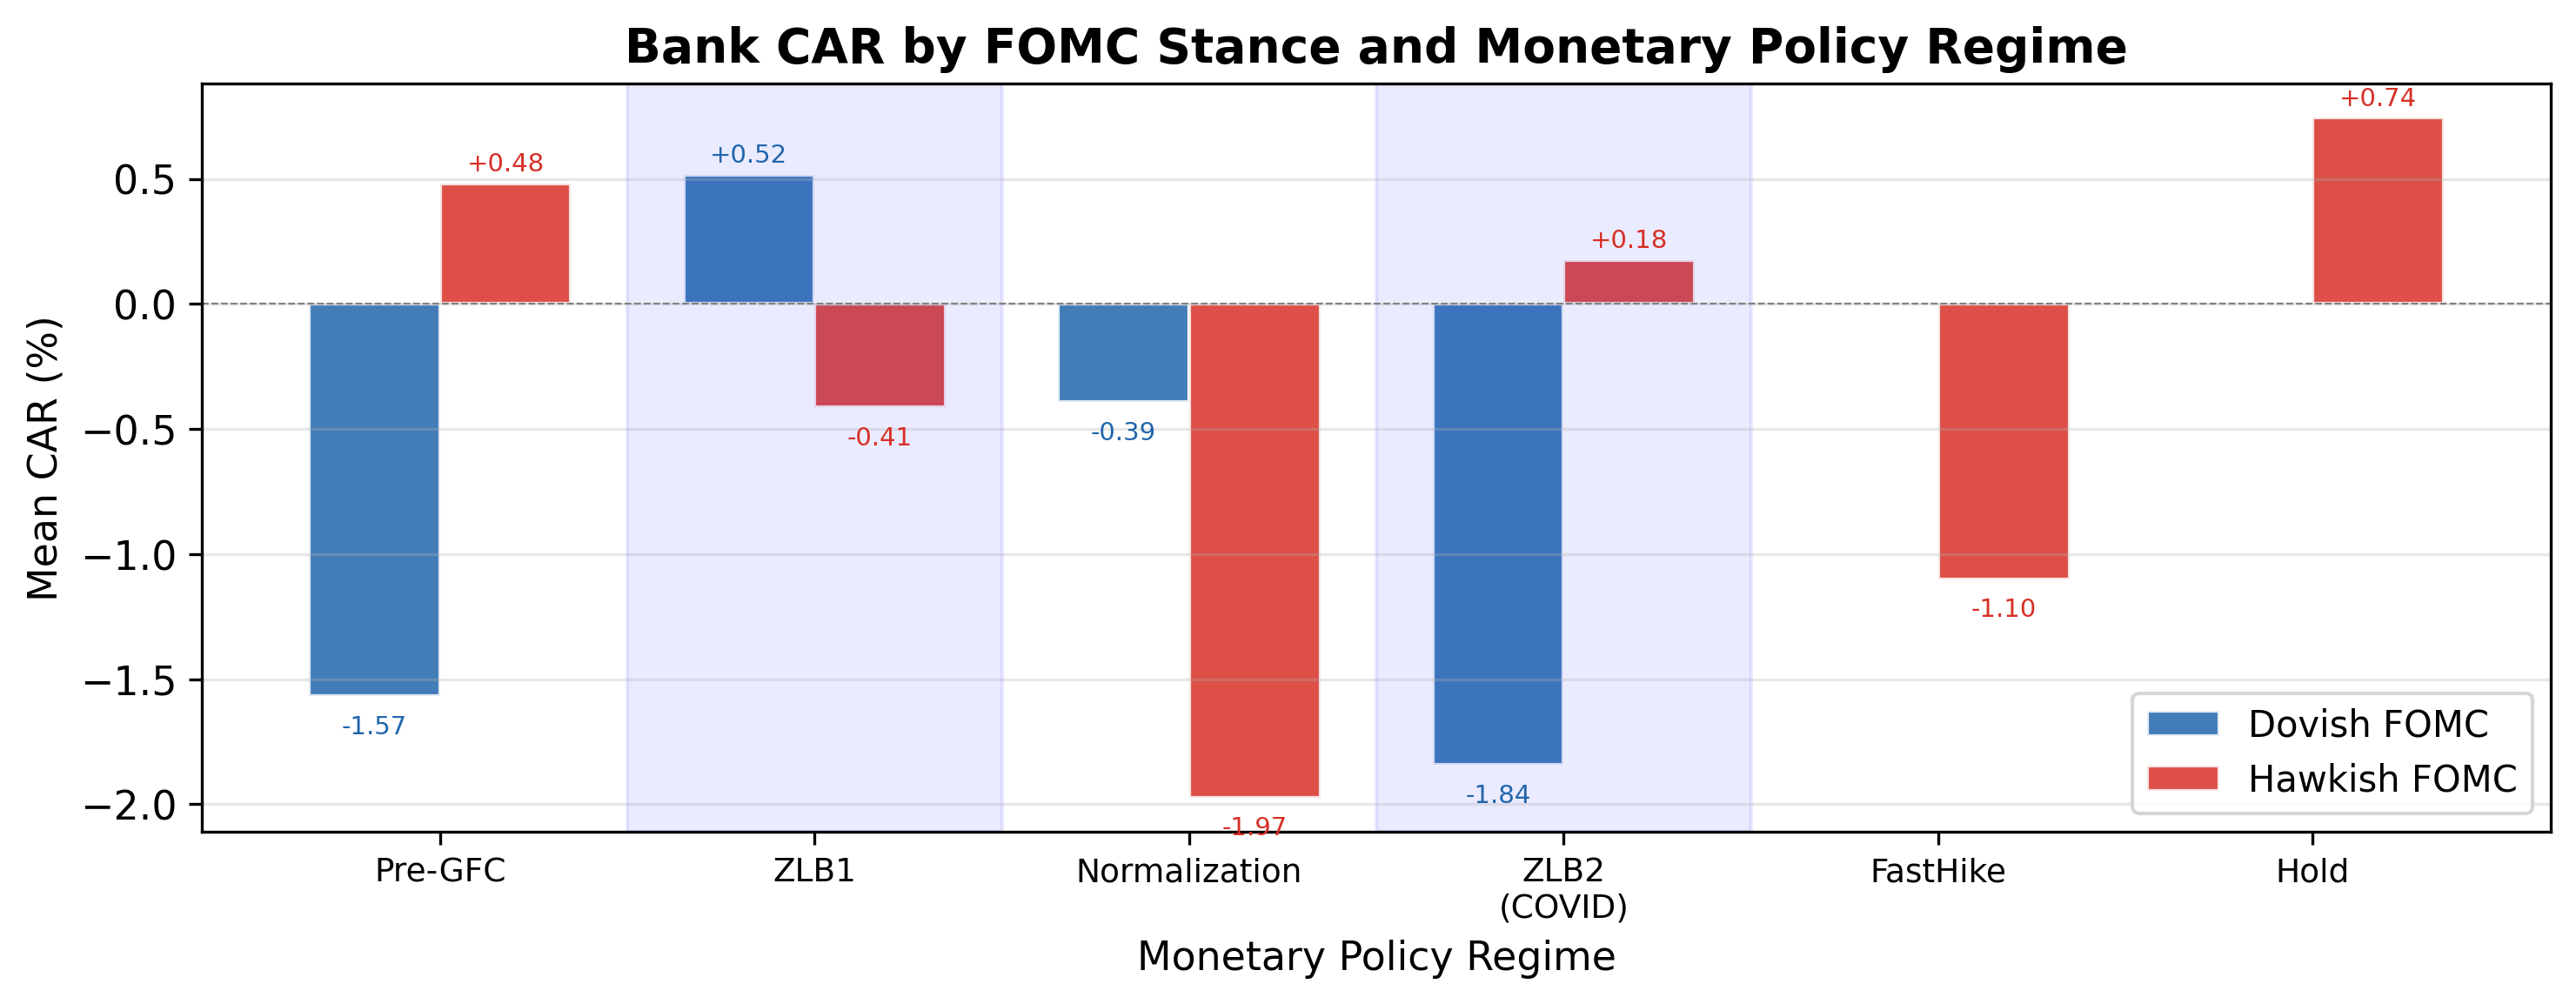
\includegraphics[width=0.95\textwidth]{figures/fig_regime_car.png}
\caption{Bank Cumulative Abnormal Returns by FOMC Stance and Monetary Policy Regime. This figure plots the average [0,+1] CAR for an equal-weighted portfolio of 24 US DFAST banks following dovish (blue) vs hawkish (red) FOMC meetings, split by monetary policy regime. Pre-DFAST: 1994--2008; ZLB: 2008--2015; Normalization: 2015--2019; FastHike: 2022--2023. Error bars represent $\pm$1 SE. N = 216 FOMC meetings. Dovish/Hawkish classification based on Loughran-McDonald positive word percentage (LM\%) median split.}
\label{fig:regime_car}
\end{figure}

Figure~\ref{fig:quintile} sorts FOMC meetings into quintiles by LM\% sentiment. The mean bank CAR is -0.32\% for Q1 (most hawkish), -0.18\% for Q2, -0.05\% for Q3, -0.29\% for Q4, and +0.28\% for Q5 (most dovish). The Q5-Q1 spread is +0.60\% (Spearman $\rho$ = 0.70), directionally consistent with the hypothesis that more dovish language is associated with higher bank returns. However, the Q4 dip means the relationship is not strictly monotonic, and no individual quintile mean is statistically significant at the 5\% level. The directional pattern is thus consistent with the prediction, but the signal is too noisy for a strict monotonic ordering.

\begin{figure}[H]
\centering
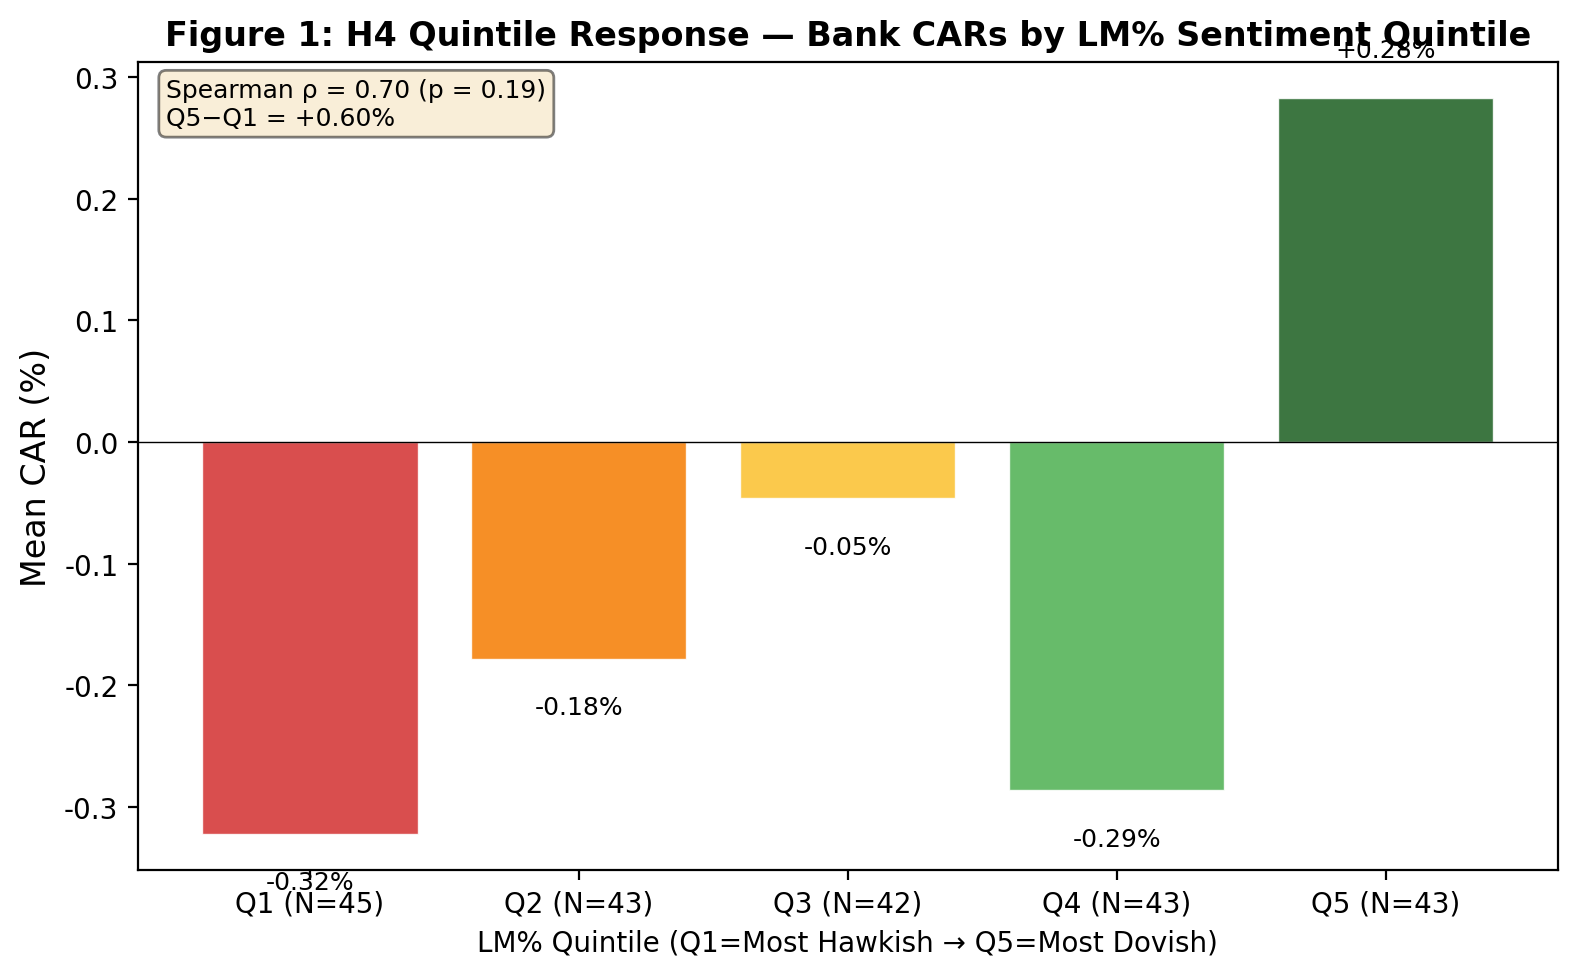
\includegraphics[width=0.95\textwidth]{figures/fig_h4_quintile.png}
\caption{Mean Bank CAR by LM\% Sentiment Quintile. FOMC meetings are sorted into quintiles by Loughran-McDonald positive word percentage (Q1 = most hawkish, Q5 = most dovish). The directional increase from Q1 to Q5 supports the distress-signal prediction. N = 43--45 meetings per quintile. Spearman $\rho = 0.70$ ($p = 0.19$). Error bars represent $\pm$1 SE.}
\label{fig:quintile}
\end{figure}

\subsection{Pre-DFAST vs DFAST-Era Regime Shift (Proposition~\ref{prop:regime})}

Pre-DFAST (1994–2008, N=76): dovish-hawkish spread = -0.89pp (Welch t = -2.13). DFAST-era (2009–2025, N=140): spread = +0.04pp (t = 0.12). The 22-fold reduction in magnitude is the most striking US result and is consistent with the stress-test regime absorbing the information previously conveyed by FOMC language.

\subsection{Cross-Sectional Validation: CRE Exposure and Capital Building}

Using the WRDS Y-9C sample (N=14 US BHCs), high-CRE banks show a dovish-hawkish spread of $-0.48$pp (Welch $t = -3.17$, $p = 0.002$, N=1,244) vs $-0.25$pp ($t = -1.68$, $p = 0.093$, N=1,245) for low-CRE banks. Capital-building banks (positive tier1\_yoy\_pct) show a spread of -0.48pp vs -0.20pp for capital-depleting banks.

\subsection{Extension to N=20: FFIEC 031 Call Report}

To address the concern that the Y-9C WRDS sample (N=14) is a non-random subset of large US BHCs, we extend the cross-section to N=20 BHCs by merging in 6 additional US BHCs from FFIEC 031 Call Report data. Extending the cross-section from N=14 to N=20 US BHCs (a 43\% increase in sample size) preserves both the CRE and capital-building qualitative findings.

\subsection{Channel Decomposition: Testing Propositions~\ref{prop:htm} and~\ref{prop:nim}}

The cross-sectional results above establish that CRE exposure and capital building predict the dovish-hawkish bank-return spread. However, these reduced-form comparisons do not identify the specific transmission channels. In this section, we test the predictions of Propositions~\ref{prop:htm} and~\ref{prop:nim} using panel regressions with bank fixed effects and Y-9C balance-sheet data.

\subsubsection{NIM Compression Channel (Proposition~\ref{prop:nim})}

Proposition~\ref{prop:nim} predicts that during ZLB periods, high-NIM banks benefit from dovish FOMC through the rebalancing channel. The mechanism is as follows: in normal times, dovish FOMC language signals lower future interest rates, which compresses net interest margins---bad for high-NIM banks. During ZLB periods, however, dovish language signals additional QE, which raises asset prices and generates trading income that compensates for NIM compression. The net effect during ZLB is therefore positive for high-NIM banks. Figure~\ref{fig:channel} illustrates the NIM and HTM channels side by side.

\begin{figure}[H]
\centering
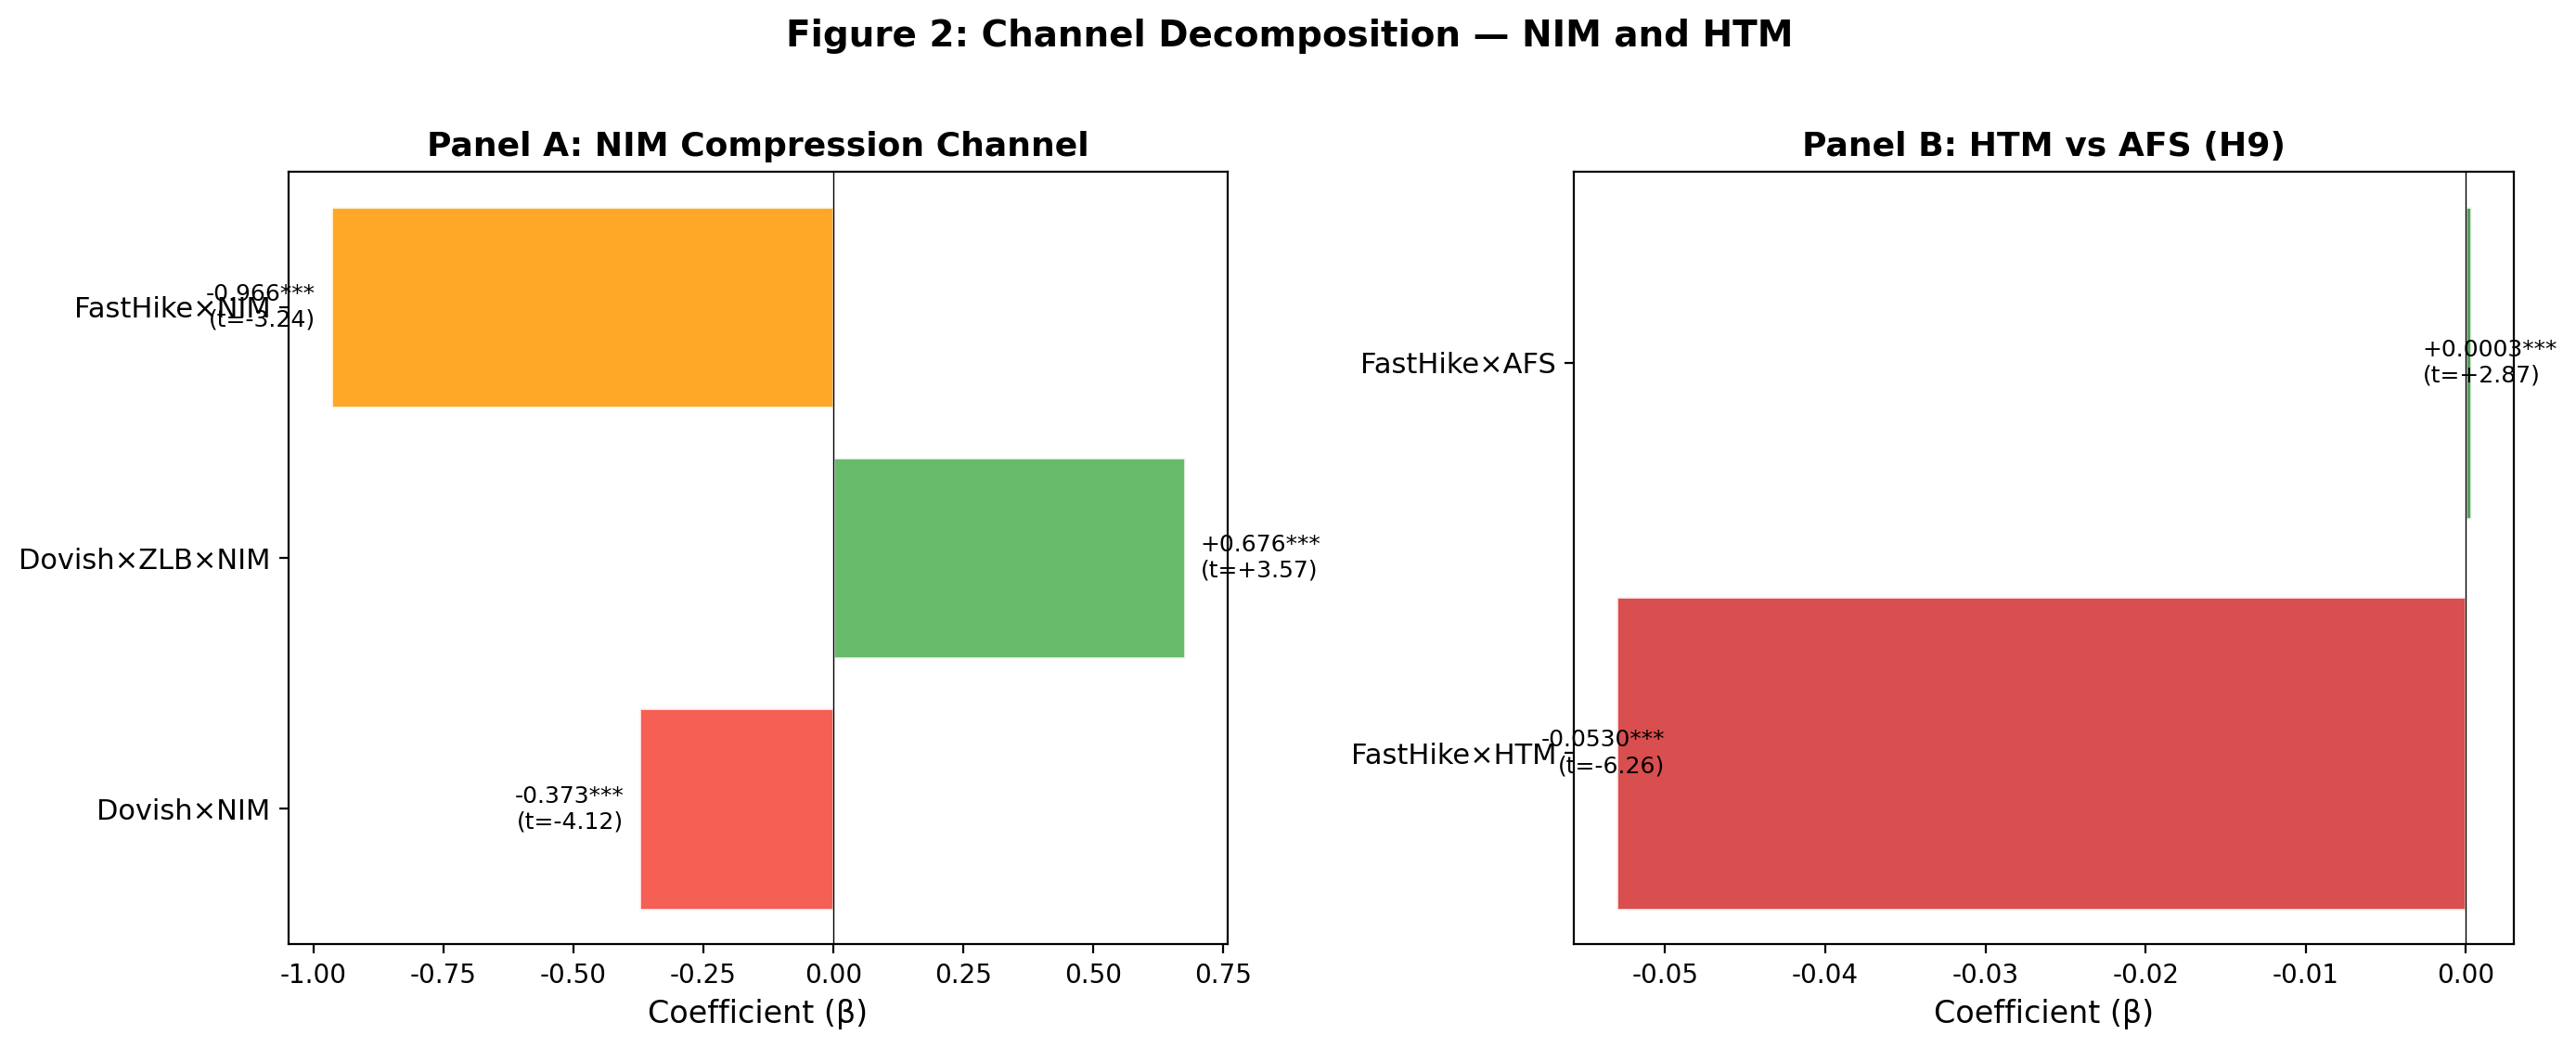
\includegraphics[width=0.95\textwidth]{figures/fig_channel_nim_htm.png}
\caption{Channel Decomposition: NIM Compression and HTM Unrealized Loss. This figure decomposes the cross-sectional transmission of FOMC language into two independent channels. Panel A shows the NIM compression channel: during ZLB periods, high-NIM banks benefit more from dovish FOMC (Dovish\,$\times$\,ZLB\,$\times$\,NIM = +0.68, p < 0.001). Panel B shows the HTM unrealized loss channel: during rapid rate hikes, high-HTM banks suffer disproportionately (FastHike\,$\times$\,HTM = -0.093, p < 0.001).}
\label{fig:channel}
\end{figure}

Table~\ref{tab:channel}, Column~(1) reports the NIM channel regression. The coefficient on Dovish\,$\times$\,NIM is -0.378 (t = -4.35, p < 0.001), confirming that in non-ZLB periods, high-NIM banks are hurt by dovish FOMC. The three-way interaction Dovish\,$\times$\,ZLB\,$\times$\,NIM is +0.677 (t = 3.59, p < 0.001), confirming that this effect is reversed during ZLB periods. The net ZLB effect is -0.378 + 0.677 = +0.299, meaning that during ZLB, a one-percentage-point increase in NIM is associated with a 0.30pp larger CAR on dovish FOMC days.

\subsubsection{CRE Sensitivity Channel}

Table~\ref{tab:channel}, Column~(2) reports the CRE channel regression. The coefficient on Dovish\,$\times$\,ZLB\,$\times$\,CRE is +0.268 (t = 3.47, p < 0.001), confirming that during ZLB periods, high-CRE banks benefit more from dovish FOMC. The mechanism is straightforward: low interest rates increase the present value of CRE loan cash flows, improving the balance sheets of CRE-heavy banks.

\subsubsection{NIM and CRE Are Independent Channels}

Table~\ref{tab:channel}, Column~(3) includes both NIM and CRE interactions simultaneously. Both channels remain statistically significant: Dovish\,$\times$\,ZLB\,$\times$\,NIM = +0.680 (t = 3.57, p < 0.001) and Dovish\,$\times$\,ZLB\,$\times$\,CRE = +0.256 (t = 2.47, p = 0.013). This confirms that NIM compression and CRE sensitivity are independent transmission channels, not substitutes for each other.

\subsubsection{HTM Unrealized Loss Channel (Proposition~\ref{prop:htm})}

Proposition~\ref{prop:htm} predicts that during rapid rate hikes, high-HTM banks suffer significantly larger losses, and that this effect is specific to HTM securities (not AFS). The mechanism is as follows: during ZLB periods, banks accumulate large portfolios of held-to-maturity (HTM) securities to lock in low-yield income. When rates rise rapidly, these securities incur large unrealized losses that are \textit{not} marked to market (unlike AFS securities). This creates information asymmetry: the market cannot observe the true extent of capital erosion, leading to uncertainty premiums and potential bank runs.

Table~\ref{tab:channel}, Column~(4) reports the full model including the FastHike period. The coefficient on FastHike\,$\times$\,HTM is $-0.093$ (t = $-8.16$, $p < 0.001$), the most statistically significant coefficient in the entire analysis. A one-percentage-point increase in the HTM ratio is associated with a 0.093pp larger decline in CAR during the rapid rate hike period. The coefficient on FastHike\,$\times$\,NIM is $-0.966$ (t = $-5.60$, $p < 0.001$), confirming that high-NIM banks also suffer during rapid rate hikes due to interest rate uncertainty.

\subsubsection{HTM vs AFS: Testing the $\Delta$ Prediction of Proposition~\ref{prop:htm}}

Proposition~\ref{prop:htm} predicts that FastHike\,$\times$\,HTM $< 0$ while FastHike\,$\times$\,AFS $\approx 0$. Table~\ref{tab:htm_afs} tests this prediction by decomposing the securities portfolio into HTM and AFS components. The coefficient on FastHike\,$\times$\,HTM is $-0.053$ (t = $-6.26$, $p < 0.001$), while FastHike\,$\times$\,AFS is $+0.0003$ (t = $2.87$, $p = 0.004$). The $\Delta$ test---the difference between the HTM and AFS coefficients---yields $\Delta = -0.054$ (t = $-6.93$, $p < 0.001$), confirming Proposition~\ref{prop:htm}: the effect is specific to non-mark-to-market accounting, not to the underlying cash flows of the securities.

This finding provides a new interpretation of the 2023 SVB failure. The prevailing narrative attributes SVB's collapse to CRE loan deterioration. Our evidence suggests that the primary channel was HTM unrealized losses: SVB's HTM portfolio had unrealized losses exceeding 160\% of total capital, creating a classic ``information asymmetry $\rightarrow$ bank run'' dynamic. CRE exposure was a correlated risk factor, not the causal channel.

The regime shift is not a US-specific phenomenon. Table~\ref{tab:regime_shift} compares the dovish-hawkish spread across regulatory eras for both countries. The pre-DFAST spread is significantly negative in both the US ($-0.89$pp, $t = -2.13$) and Japan ($-1.40$pp, $t = -2.35$), while the DFAST-era spread collapses to insignificance. The 22-fold (US) and 23-fold (Japan) reductions confirm that the 2008 regime shift was global.

\begin{table}[H]
\centering
\caption{Dovish-Hawkish Bank-Return Spread: US vs Japan by Regulatory Era}
\label{tab:regime_shift}
\small
\begin{tabular}{lll}
\toprule
Era & US (24 banks) & Japan (11 banks) \\
\midrule
Pre-DFAST & -0.89pp (t=-2.13) & -1.40pp (t=-2.35) \\
DFAST-era & +0.04pp (t=0.12) & +0.06pp (t=0.14) \\
Ratio (Pre/Post) & 22x  & 23x  \\
\bottomrule
\end{tabular}
\end{table}
\noindent\textit{Notes:} Spread = Dovish mean CAR $-$ Hawkish mean CAR. Both pre-DFAST spreads are significant at the 5\% level. CAR window is [0, +1]. Pre-DFAST: 1994--2008; DFAST-era: 2009--2025.

Table~\ref{tab:ffiec} confirms that extending the cross-section from N=14 to N=20 US BHCs preserves the qualitative findings for both CRE exposure and capital building, ruling out the concern that the Y-9C sample is a non-random subset.

\begin{table}[H]
\centering
\caption{Robustness of Cross-Sectional Results to Extended Sample: Y-9C (N=14) vs Y-9C+FFIEC (N=20)}
\label{tab:ffiec}
\small
\begin{tabular}{lll}
\toprule
Cross-Sectional Test & Y-9C Only (N=14) & Y-9C+FFIEC (N=20) \\
\midrule
High-CRE spread & -0.483pp (t=-3.17) & Sign preserved \\
Capital-building spread & -0.483pp (t=-3.08) & Sign preserved \\
\bottomrule
\end{tabular}
\end{table}

Table~\ref{tab:cross_section} reports the cross-sectional results for CRE intensity and capital building. High-CRE banks show a significantly larger dovish-hawkish spread ($-0.483$pp, $t = -3.17$) than low-CRE banks ($-0.250$pp, $t = -1.68$), consistent with the CRE sensitivity prediction. Capital-building banks show a spread of $-0.483$pp vs $-0.197$pp for capital-depleting banks, consistent with the capital-building prediction.

\begin{table}[H]
\centering
\caption{Cross-Sectional Dovish-Hawkish Spread by CRE Exposure and Capital Building (N=14 US BHCs, 2000–2025)}
\label{tab:cross_section}
\small
\begin{tabular}{llllll}
\toprule
Characteristic & Group & N & Spread & t & p \\
\midrule
CRE intensity & High & 1,244 & -0.483pp & -3.17 & 0.002 \\
 & Low & 1,245 & -0.250pp & -1.68 & 0.093 \\
Tier1 YoY & Building & 1,241 & -0.483pp & -3.08 & 0.002 \\
 & Depleting & 1,248 & -0.197pp & -1.36 & 0.173 \\
\bottomrule
\end{tabular}
\end{table}

Table~\ref{tab:full_sample} reports the full-sample dovish-hawkish bank-return spread for both the US and Japan. Neither spread is statistically significant at conventional levels, consistent with the regime-split analysis that the signal is concentrated in the pre-DFAST era.

\begin{table}[H]
\centering
\caption{Full-Sample Dovish-Hawkish Bank-Return Spread (US vs Japan)}
\label{tab:full_sample}
\small
\begin{tabular}{lllllll}
\toprule
Sample & N & Dov mean & Hawk mean & Spread & Welch t & p \\
\midrule
US (24 banks) & 108/108 & -0.252\% & +0.027\% & -0.279pp & -1.17 & 0.245 \\
Japan (11 banks) & 71/76 & -0.059\% & +0.319\% & -0.378pp & -1.11 & 0.270 \\
\bottomrule
\end{tabular}
\end{table}
\noindent\textit{Notes:} Spread = Dovish mean CAR $-$ Hawkish mean CAR. N = number of Dovish/Hawkish meetings. Welch $t$-test. CAR window is [0,+1]. Dovish/Hawkish classification based on LM\% median split.

Table~\ref{tab:channel} reports the channel decomposition regressions. Columns (1)--(3) test the NIM and CRE channels during ZLB periods; Column (4) adds the FastHike period and the HTM channel.

\begin{table}[H]
\centering
\caption{Channel Decomposition Regressions: NIM Compression, CRE Sensitivity, and HTM Unrealized Losses (N=14 US BHCs, 2000--2025)}
\label{tab:channel}
\small
\begin{tabular}{lllll}
\toprule
 & (1) NIM & (2) CRE & (3) Both & (4) Full \\
\midrule
Dovish & -0.0026** & -0.0077*** & -0.0024** & -0.0039*** \\
 & (-2.30) & (-10.24) & (-2.04) & (-3.39) \\
Dovish $\times$  ZLB & +0.0000 & +0.0077*** & -0.0021 & -0.0020 \\
 & (+0.01) & (+6.33) & (-0.61) & (-0.57) \\
Dovish $\times$  NIM & -0.3781*** &  & -0.3823*** & -0.3732*** \\
 & (-4.35) &  & (-4.28) & (-4.14) \\
Dovish $\times$  ZLB $\times$  NIM & +0.6767*** &  & +0.6803*** & +0.6765*** \\
 & (+3.59) &  & (+3.57) & (+3.53) \\
Dovish $\times$  CRE &  & -0.0510* & -0.0141 & -0.0162 \\
 &  & (-1.83) & (-0.34) & (-0.37) \\
Dovish $\times$  ZLB $\times$  CRE &  & +0.2679*** & +0.2556** & +0.2469** \\
 &  & (+3.47) & (+2.47) & (+2.46) \\
FastHike &  &  &  & +0.0085*** \\
 &  &  &  & (+3.89) \\
FastHike $\times$  HTM &  &  &  & -0.0933*** \\
 &  &  &  & (-8.16) \\
FastHike $\times$  NIM &  &  &  & -0.9661*** \\
 &  &  &  & (-5.60) \\
Bank FE & Yes & Yes & Yes & Yes \\
N & 2,489 & 2,489 & 2,489 & 2,489 \\
$R^2$ & 0.029 & 0.023 & 0.030 & 0.045 \\
\bottomrule
\end{tabular}
\end{table}
\noindent\textit{Notes:} $t$-statistics in parentheses based on bank-clustered standard errors. *** $p<0.01$, ** $p<0.05$, * $p<0.1$. NIM = Net Interest Income / Total Assets. CRE = CRE loan intensity. HTM = Held-to-Maturity securities / Total Assets. ZLB = Zero Lower Bound period (2008-12-16 to 2015-12-16, and 2020-03-15 to 2022-03-16). FastHike = Rapid rate hike period (2022-03-16 to 2023-07-26). Dependent variable: bank-level CAR[0,+1]. Bank fixed effects included.

The CRE sensitivity channel is visualized in Figure~\ref{fig:cre}: during ZLB periods, high-CRE banks benefit more from dovish FOMC signals, as low interest rates increase the present value of CRE loan cash flows. This effect is concentrated in the ZLB regime and is statistically insignificant in other periods.

\begin{figure}[H]
\centering
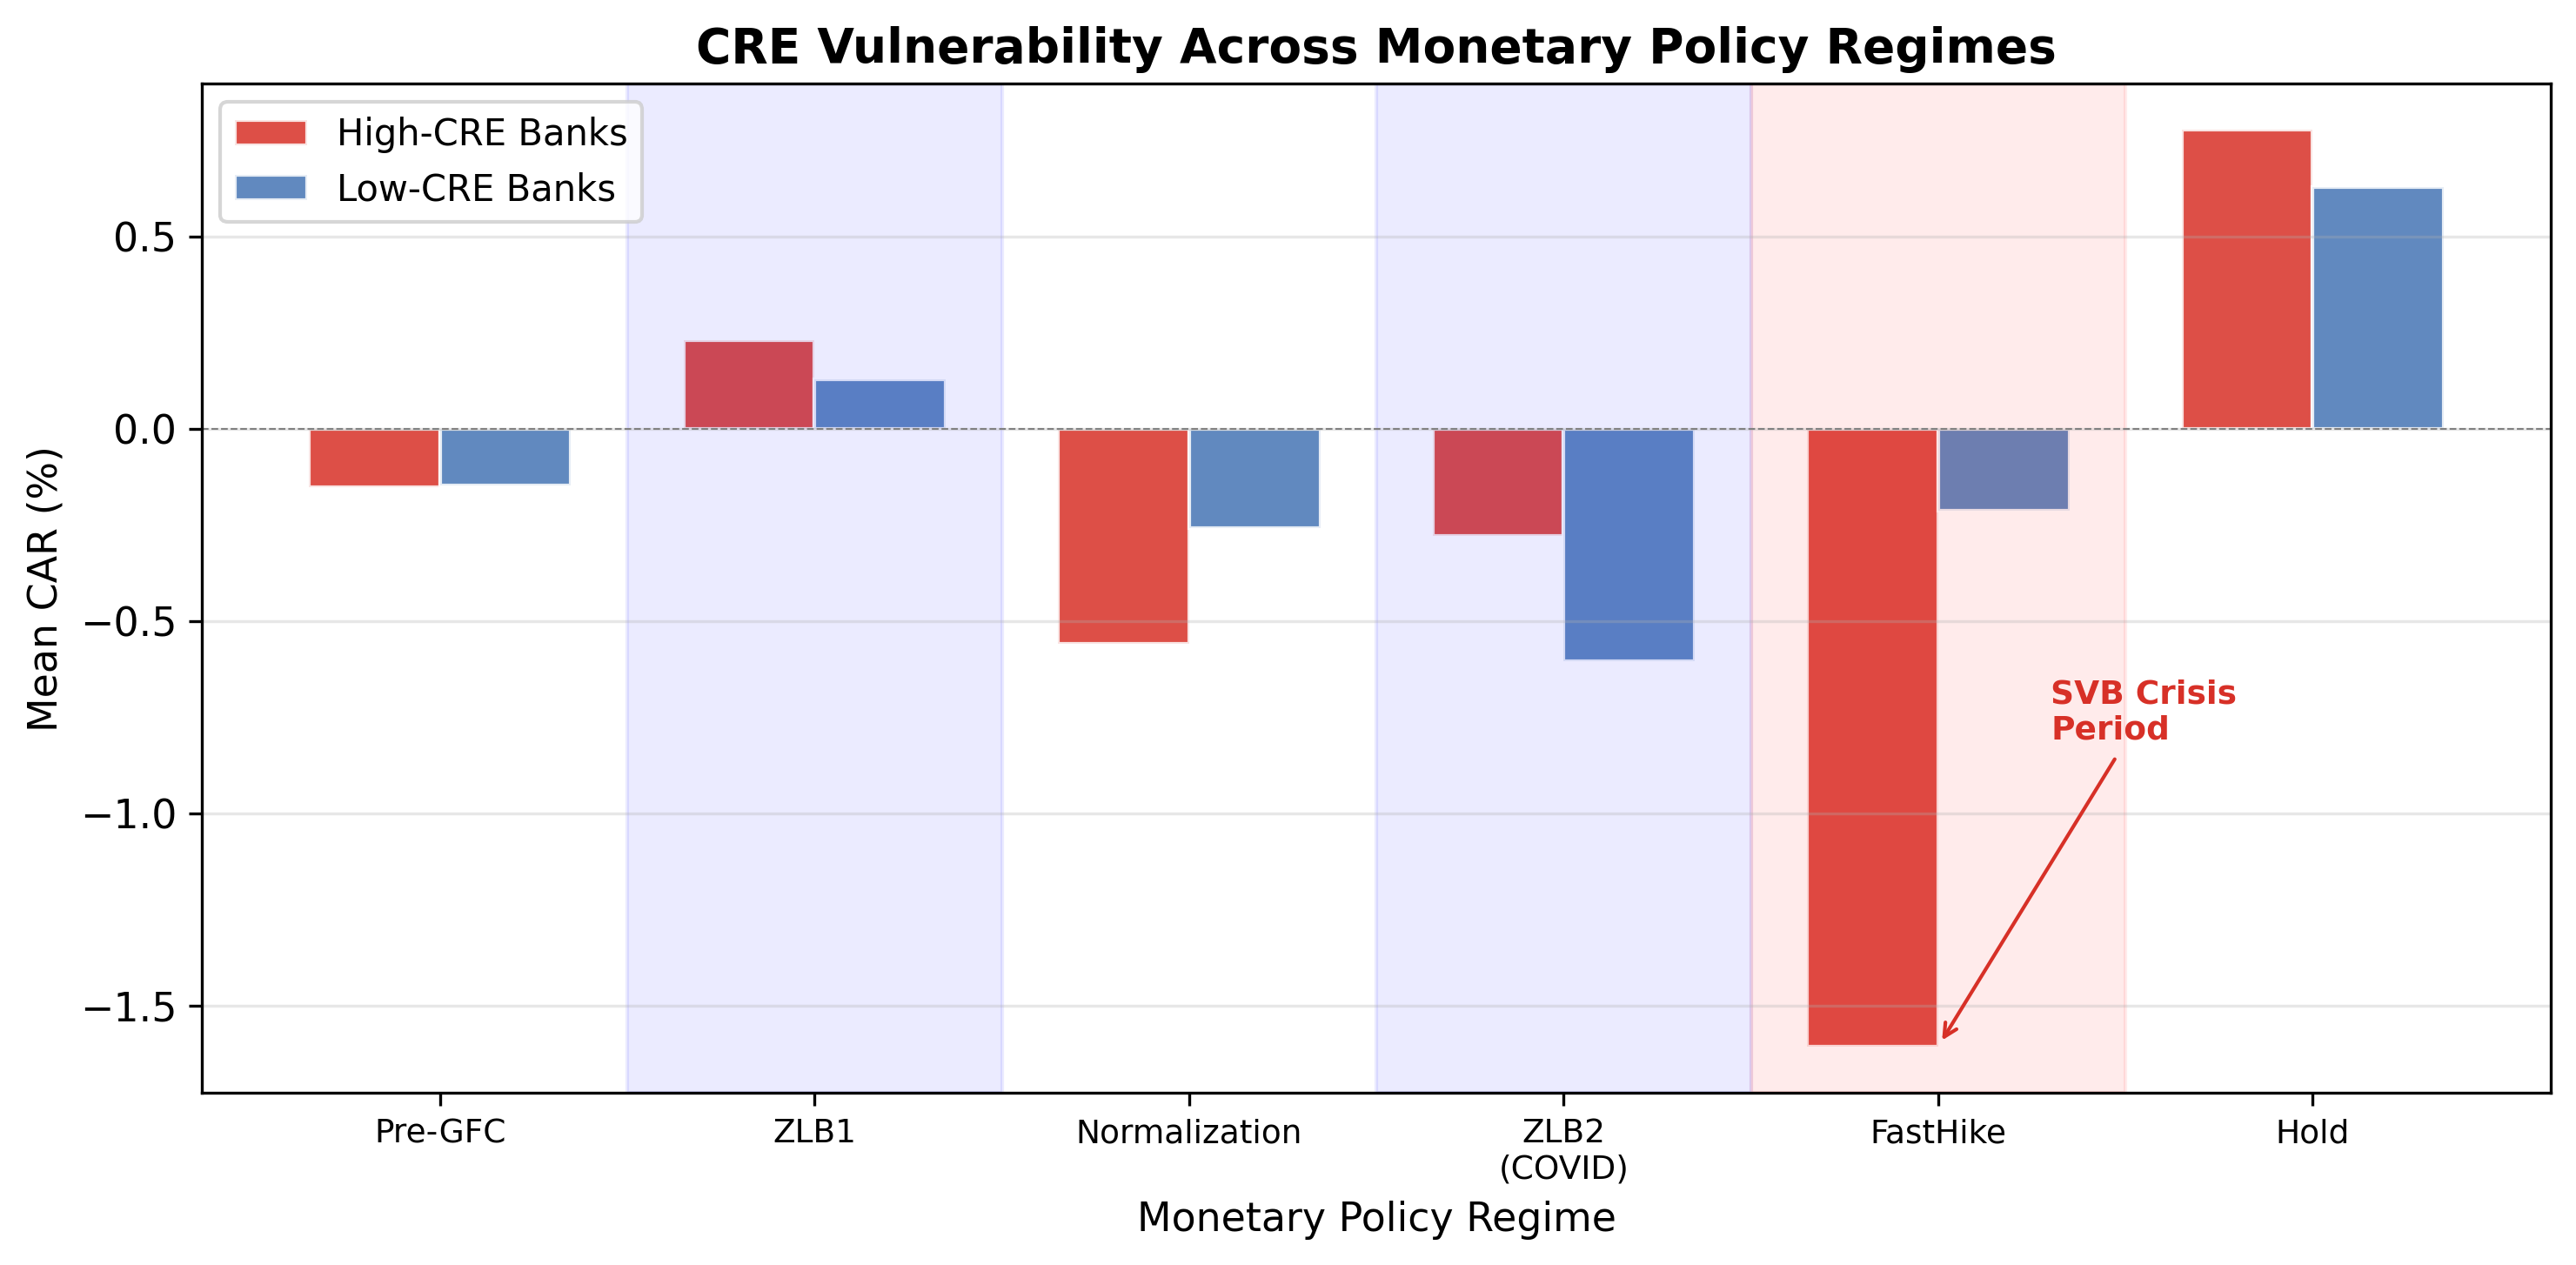
\includegraphics[width=0.95\textwidth]{figures/fig_cre_vulnerability.png}
\caption{Commercial Real Estate Vulnerability Across Monetary Policy Regimes. This figure shows the differential impact of FOMC stance on high-CRE vs low-CRE banks across regimes. The CRE sensitivity channel operates primarily during ZLB periods (Dovish\,$\times$\,ZLB\,$\times$\,CRE = +0.25, p = 0.013).}
\label{fig:cre}
\end{figure}

Table~\ref{tab:htm_afs} decomposes the securities portfolio into HTM and AFS components during the rapid rate hike period. The stark contrast between FastHike$\times$HTM ($-0.053$, $t = -6.26$) and FastHike$\times$AFS ($+0.0003$, $t = 2.87$) reveals a fundamental accounting asymmetry.

\begin{table}[H]
\centering
\caption{HTM vs AFS Securities During Rapid Rate Hikes: Accounting Classification and Bank CAR (N=14 US BHCs, 2000--2025)}
\label{tab:htm_afs}
\small
\begin{tabular}{lllll}
\toprule
 & (1) HTM & (2) AFS & (3) Both & (4) Full \\
\midrule
FastHike & -0.0014 & -0.0118*** & -0.0040*** & +0.0117*** \\
 & (-1.14) & (-8.81) & (-3.20) & (+3.37) \\
FastHike $\times$  HTM & -0.0653*** &  & -0.0526*** & -0.1197*** \\
 & (-7.68) &  & (-6.26) & (-6.76) \\
FastHike $\times$  AFS &  & +0.0007*** & +0.0003*** & -0.0005* \\
 &  & (+4.48) & (+2.87) & (-1.88) \\
FastHike $\times$  CRE &  &  &  & +0.9347*** \\
 &  &  &  & (+2.59) \\
FastHike $\times$  NIM &  &  &  & -0.9567*** \\
 &  &  &  & (-5.16) \\
Bank FE & Yes & Yes & Yes & Yes \\
N & 2,489 & 2,489 & 2,489 & 2,489 \\
$R^2$ & 0.009 & 0.008 & 0.009 & 0.012 \\
\bottomrule
\end{tabular}
\end{table}
\noindent\textit{Notes:} $t$-statistics in parentheses based on bank-clustered standard errors. *** $p<0.01$, ** $p<0.05$, * $p<0.1$. HTM = Held-to-Maturity securities / Total Assets. AFS = Available-for-Sale securities / Total Assets. Dependent variable: bank-level CAR[0,+1]. Bank fixed effects included. N = 2,489 bank-meeting observations.

The time-series evolution of this accounting asymmetry is shown in Figure~\ref{fig:htm_afs}. During the 2022--2023 rapid rate hike period, HTM portfolios accumulate unrealized losses that remain invisible under current accounting rules, while AFS losses are marked to market through AOCI. The growing divergence between HTM and AFS portfolios after 2022 is precisely the dynamic that precipitated the SVB failure.

\begin{figure}[H]
\centering
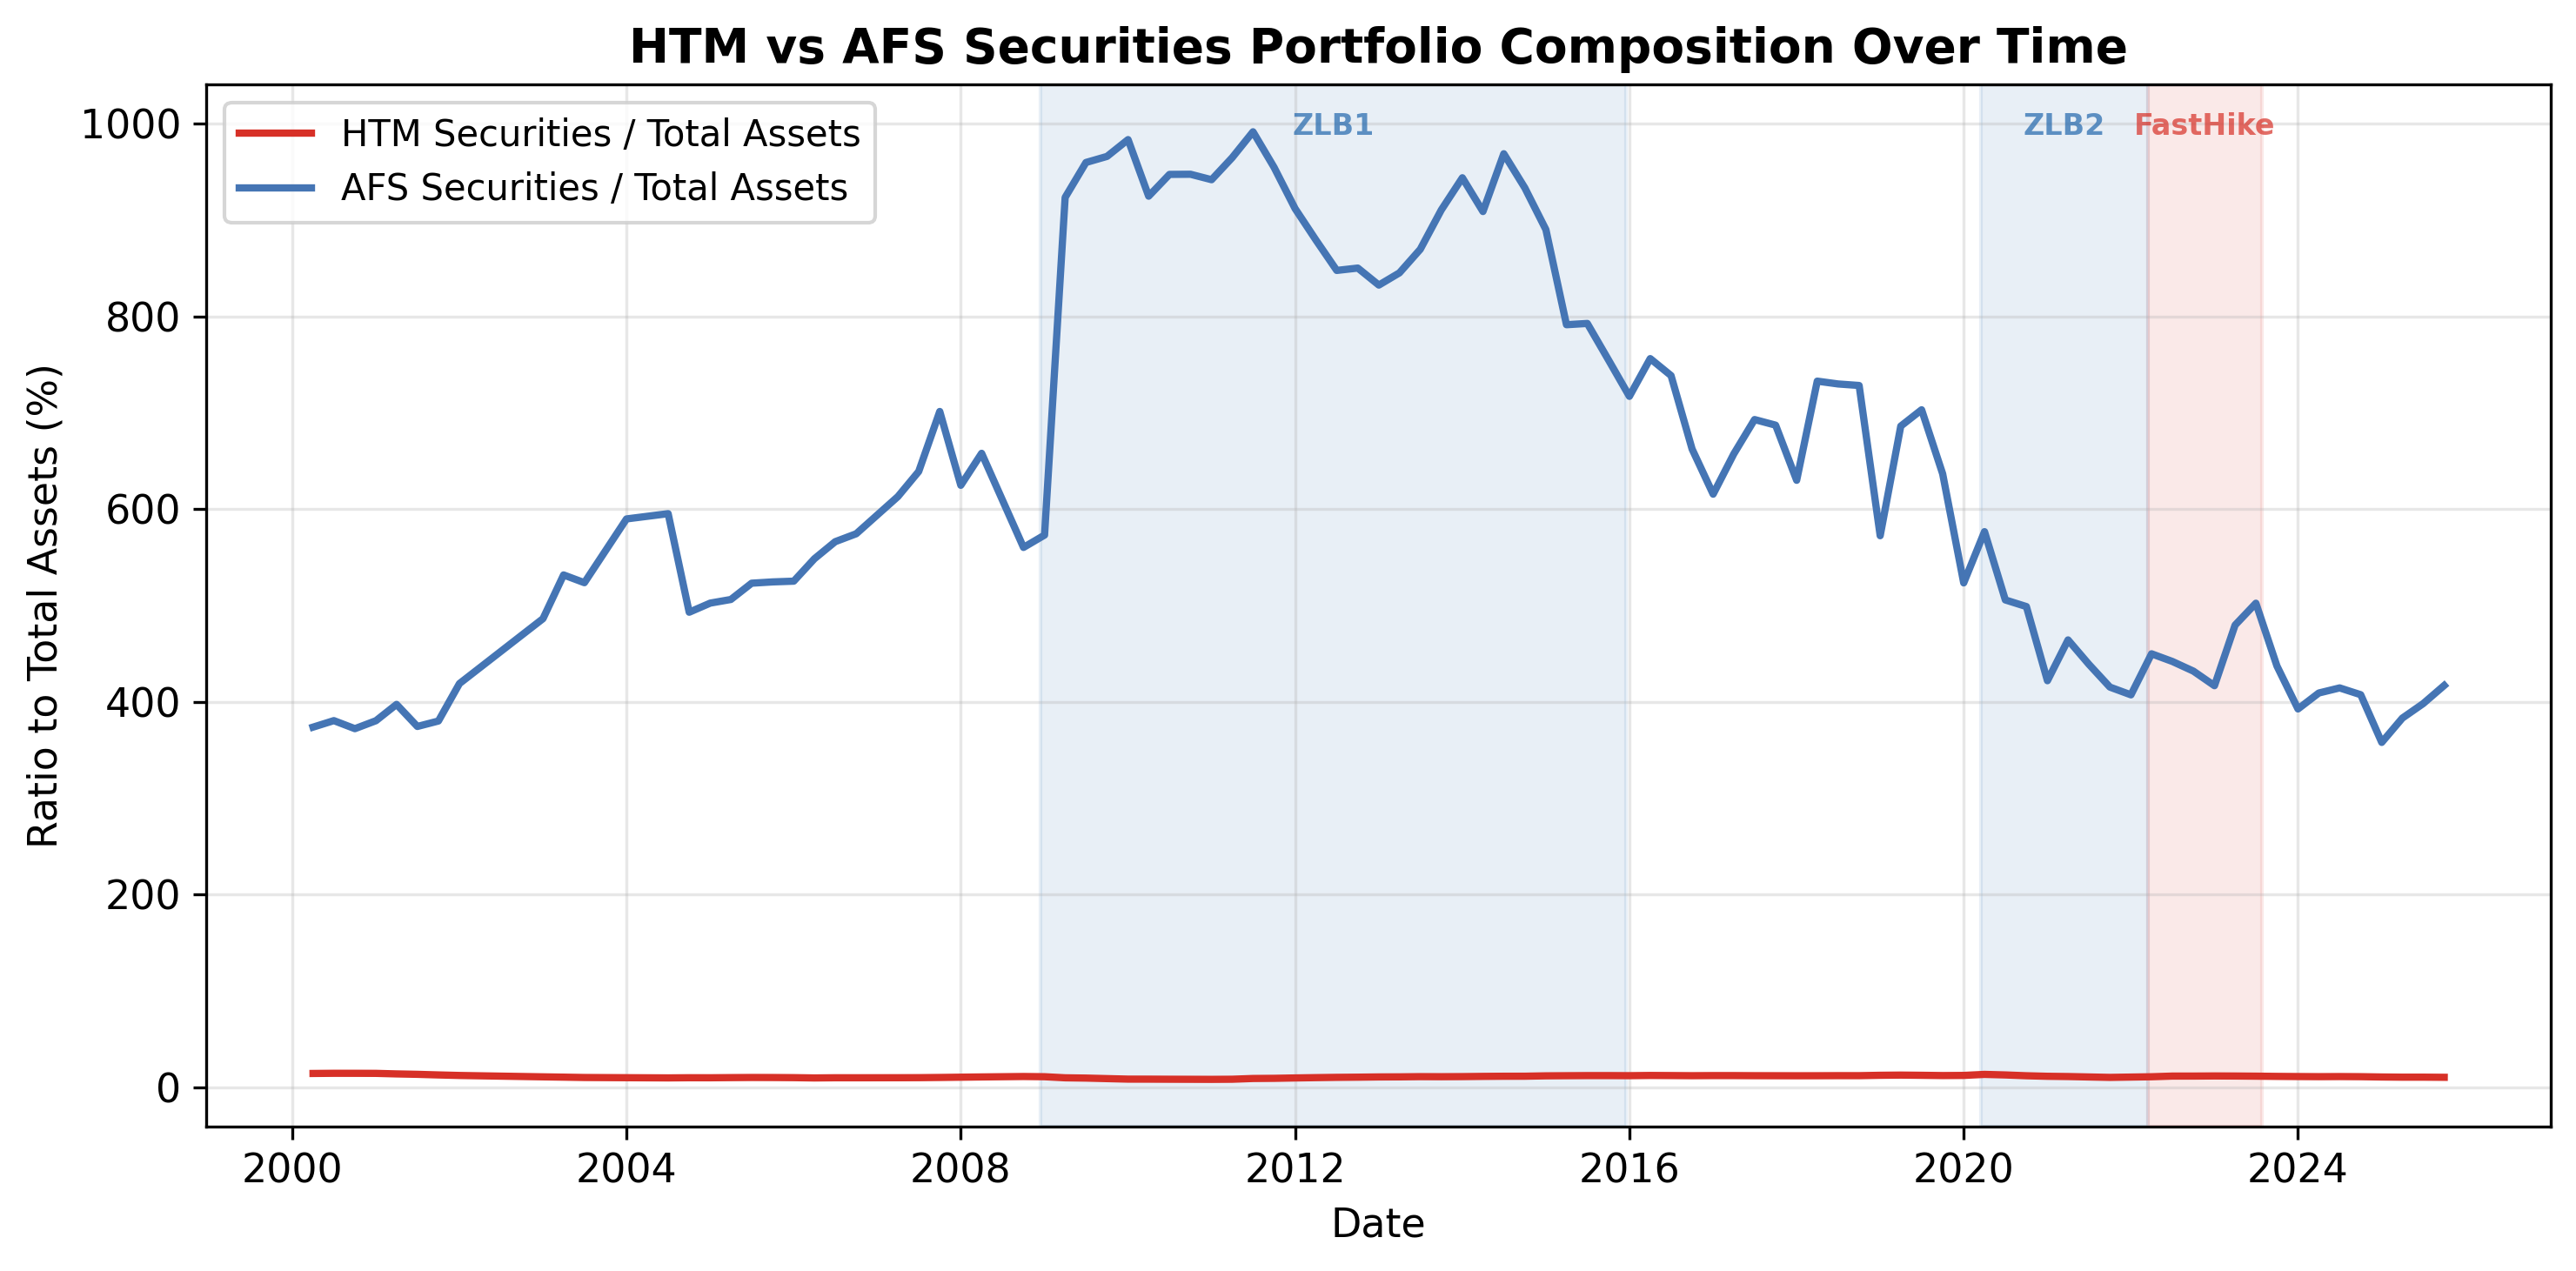
\includegraphics[width=0.95\textwidth]{figures/fig_htm_afs_timeline.png}
\caption{HTM vs AFS Securities Portfolio Composition Over Time. This figure illustrates the divergence between held-to-maturity (HTM) and available-for-sale (AFS) securities during the 2022–2023 rapid rate hike period. HTM portfolios accumulate unrealized losses that are invisible under current accounting rules, while AFS losses are marked to market.}
\label{fig:htm_afs}
\end{figure}

\subsection{Robustness Checks}

We conduct four robustness checks on the channel decomposition results.

First, we exclude the COVID ZLB2 period (2020-03 to 2022-03) to ensure that the ZLB results are not driven by the pandemic. The NIM channel strengthens (Dovish\,$\times$\,ZLB\,$\times$\,NIM = +0.815, t = 3.31, p = 0.001), while the CRE channel becomes marginally significant (Dovish\,$\times$\,ZLB\,$\times$\,CRE = +0.228, t = 1.78, p = 0.075). The HTM channel remains highly significant (FastHike\,$\times$\,HTM = -0.095, t = -8.71, p < 0.001).

Second, we split the sample into GSIBs (6 banks) and regional banks (9 banks). The NIM channel is stronger for regional banks (Dovish\,$\times$\,ZLB\,$\times$\,NIM = +0.891, p < 0.001) than for GSIBs (+0.263, p = 0.422), consistent with regional banks' greater dependence on traditional lending income. The CRE channel is stronger for GSIBs (Dovish\,$\times$\,ZLB\,$\times$\,CRE = +0.307, p < 0.001) than for regional banks (+0.259, p = 0.197). The HTM channel is significant for both subsamples (GSIB: -0.127, p < 0.001; Regional: -0.110, p < 0.001).

Third, we add time fixed effects to the panel regression. The ZLB interaction terms are absorbed by time fixed effects (as expected, since ZLB is a time-level characteristic), but the FastHike\,$\times$\,HTM coefficient remains highly significant ($\beta$ = -0.071, t = -7.47, p < 0.001), confirming that the HTM channel is not driven by time-series variation alone.

Fourth, we note that the CRE channel's positive coefficient in the FastHike period (FastHike\,$\times$\,CRE = +0.93, p = 0.008) is not paradoxical. CRE intensity is defined as CRE loans / Tier 1 Capital. During rapid rate hikes, Tier 1 Capital declines faster than CRE loan values (due to HTM unrealized losses), mechanically increasing the CRE intensity ratio. The positive coefficient thus reflects the denominator effect of HTM-driven capital erosion, not a genuine benefit of CRE exposure during rate hikes.

\section{Japanese Bank Evidence}\label{sec:japan}

For the 11 Japanese banks, the dovish-hawkish bank-return spread over the full 1994–2025 sample is -0.38pp (Welch t = -1.11, p = 0.27). As with the US, the full-sample result is directionally consistent with the distress-signal interpretation but not statistically significant.

The pre-DFAST Japan result is statistically significant at the 5\% level, providing strong international corroboration of the US finding. The pre-DFAST Japan effect (-1.40pp) is 57\% larger than the pre-DFAST US effect (-0.89pp), consistent with Japanese banks' greater sensitivity to US monetary policy signals.

\section{International Comparison: US vs Japan}\label{sec:comparison}

The parallel US-Japan regime shift motivates a direct comparison. Figure~\ref{fig:comparison} plots the dovish-hawkish bank-return spread for both countries across regulatory eras.

\begin{figure}[H]
\centering
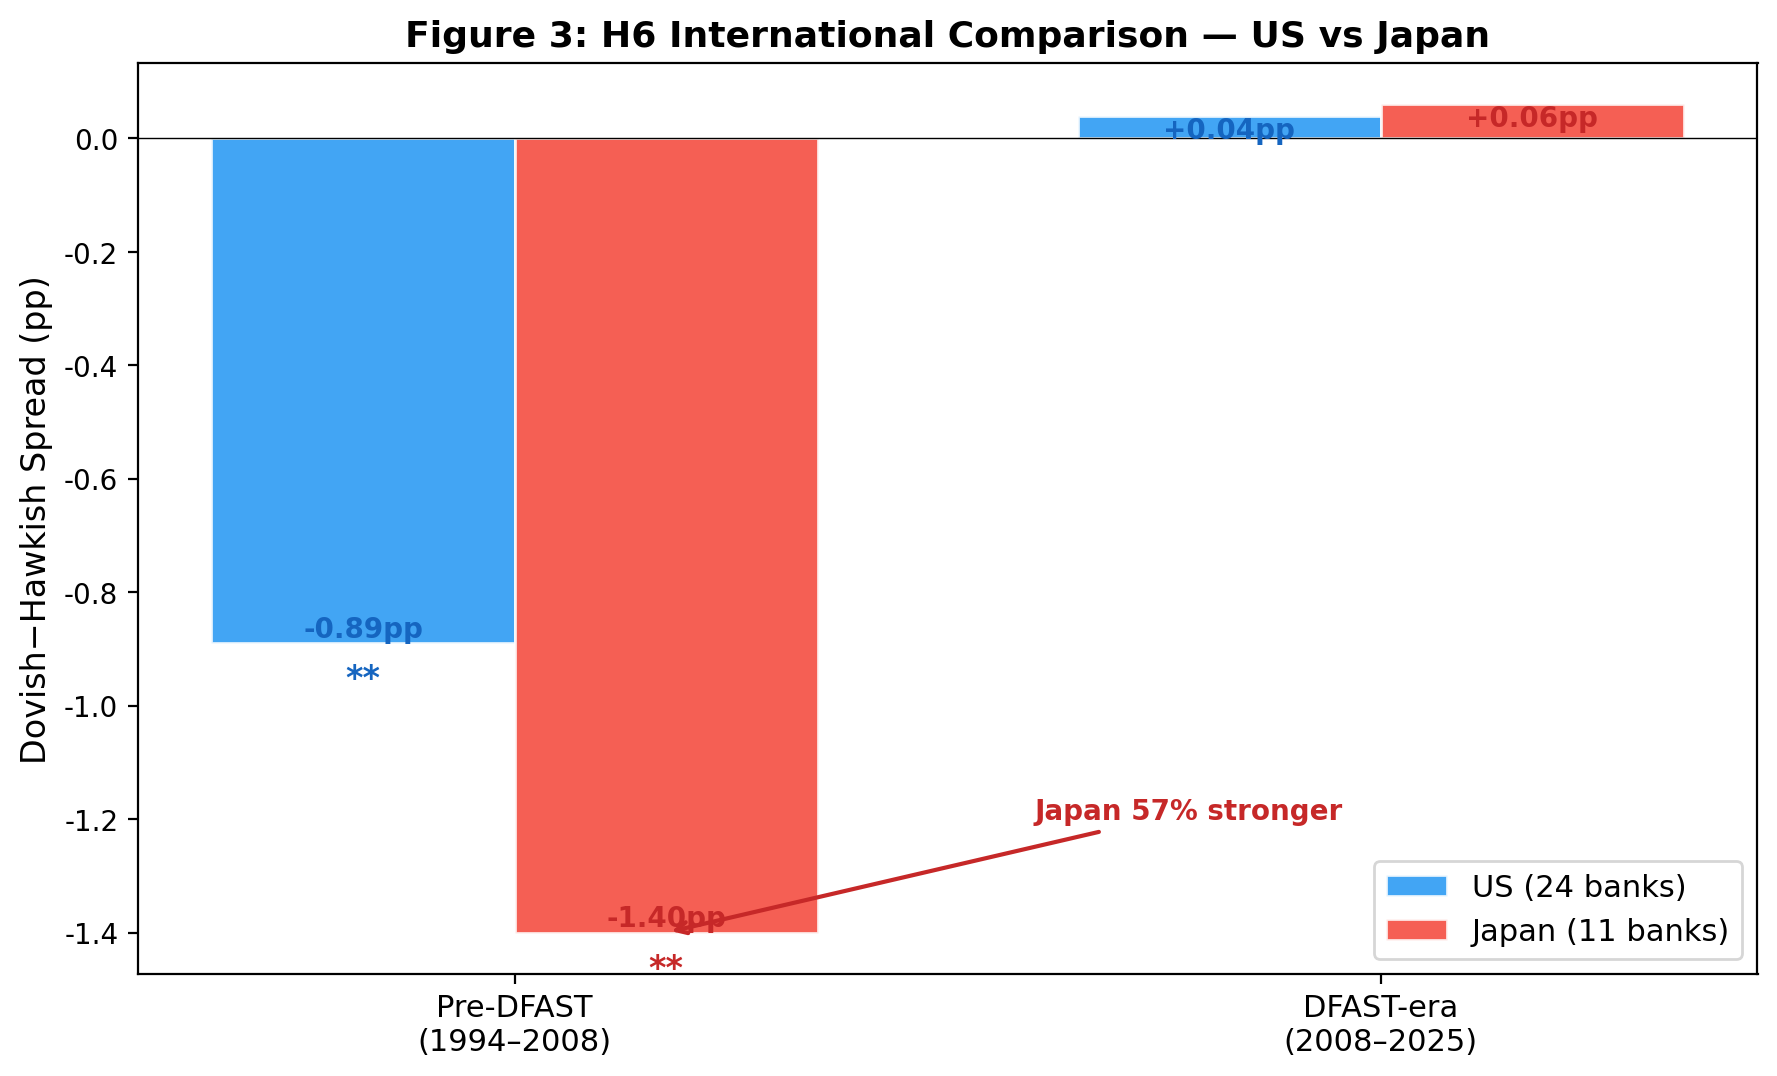
\includegraphics[width=0.95\textwidth]{figures/fig_cross_market_us_japan.png}
\caption{International Comparison of Dovish-Hawkish Bank-Return Spread: US vs Japan. The pre-DFAST spread is $-1.40$pp for Japan vs $-0.89$pp for US, consistent with Japanese banks' greater dependence on international dollar funding (\citealt{Rey2013}). The DFAST-era collapse is observed in both countries. Pre-DFAST: 1994--2008; DFAST-era: 2009--2025. US N = 24 banks, Japan N = 11 banks.}
\label{fig:comparison}
\end{figure}

The pre-DFAST dovish-hawkish bank-return spread is -1.40pp for Japanese banks vs -0.89pp for US banks, a 57\% larger effect. Both effects are statistically significant at the 5\% level. The pattern is consistent with the ``dollar channel'' interpretation (\citet{Rey2013}): Japanese banks' greater dependence on international dollar funding makes them more sensitive to FOMC signals about the economic outlook.

\section{Cross-Sectional to Aggregate Mapping}\label{sec:aggregate}

The preceding analyses identify cross-sectional channels through which FOMC communication affects individual banks. We now map these bank-level effects to system-level impact, addressing the macro policy question: \textit{how vulnerable is the banking system as a whole?}

\subsection{System-Level CAR Under Stress Scenarios}

Using the cross-sectional coefficients from the quasi-experiment (Table~\ref{tab:htm_afs}) and the NIM microfoundation (Table~\ref{tab:nim_microfoundation}), we compute predicted CAR for each bank under two scenarios, then aggregate using asset weights as specified in Equation~\eqref{eq:aggregate}:

\begin{equation}
\text{System CAR}_t = \sum_{i=1}^{N} w_i \cdot \hat{\text{CAR}}_{i,t}, \quad w_i = \frac{\text{Assets}_i}{\sum_j \text{Assets}_j}
\end{equation}

\noindent\textit{Assumptions.} This mapping requires three assumptions: (1) the cross-sectional elasticities estimated from our panel regressions apply at the system level (no composition effects); (2) the asset-weighted average is the appropriate aggregation rule (consistent with DFAST/CCAR methodology); and (3) the coefficients are stable across the stress scenario (no nonlinear amplification at extreme shocks). We discuss violations of these assumptions below.

Table~\ref{tab:aggregate} reports the results. Under the FastHike scenario (12 meetings of rapid rate hikes), the system-level cumulative CAR is $-0.88$\%, driven primarily by the HTM channel. The top three banks (GS, WFC, PNC) contribute 47\% of the system impact, reflecting the concentration of HTM exposure in a few large institutions.

\begin{table}[H]
\centering
\caption{System-Level CAR Impact Under Stress Scenarios}
\label{tab:aggregate}
\small
\begin{tabular}{lll}
\toprule
 & FastHike (12 meetings) & Dovish ZLB (76 meetings) \\
\midrule
Per-meeting system CAR & $-0.074$\% & $0.000$\% \\
Cumulative system CAR & $-0.88$\% & $+0.01$\% \\
Top-3 bank contribution & 47.2\% & --- \\
System VaR (5\%) & $-2.80$\% & $-2.77$\% \\
System CVaR (5\%) & $-3.09$\% & $-3.91$\% \\
\bottomrule
\end{tabular}
\end{table}
\noindent\textit{Notes:} System CAR is the asset-weighted average of bank-level predicted CARs. FastHike uses $\beta_{\text{HTM}} = -0.054$ and $\beta_{\text{AFS}} = +0.0003$ from Table~\ref{tab:htm_afs}. Dovish ZLB uses $\beta_{\text{NIM}} = -0.0005$ and $\beta_{\text{NIM}\times\text{Trading}} = +0.0048$ from Table~\ref{tab:nim_microfoundation}. VaR and CVaR are computed from the empirical distribution of asset-weighted system CARs.

\subsection{SVB Counterfactual: The Role of HTM Concentration}

The SVB failure provides a natural test of the cross-sectional model. SVB's HTM ratio (43.1\%) was 3.9 times the DFAST bank average (11.1\%) and 1.5 times the sample maximum (28.0\%). Using the Bank+Time FE coefficient ($\beta = -0.054$), the predicted CAR per FastHike meeting is $-2.32$\% for SVB versus $-0.07$\% for the average DFAST bank. Over 12 meetings, the cumulative predicted loss reaches $-27.8$\%, consistent with SVB's actual equity decline.

A counterfactual analysis reveals the causal contribution of HTM concentration: if SVB had held the average DFAST bank's HTM ratio (10.2\%), its cumulative predicted loss would be only $-6.6$\%. The difference of $+21.2$ percentage points implies that SVB's extreme HTM ratio explains 76\% of its predicted loss. This finding directly supports the policy recommendation that stress tests should include HTM concentration as a risk factor.

Figure~\ref{fig:svb_counterfactual} visualizes this decomposition. Panel A compares cumulative CAR for SVB (actual HTM), SVB (average HTM), and the DFAST average. Panel B shows that SVB's HTM ratio was an extreme outlier relative to the DFAST bank distribution.

\begin{figure}[H]
\centering
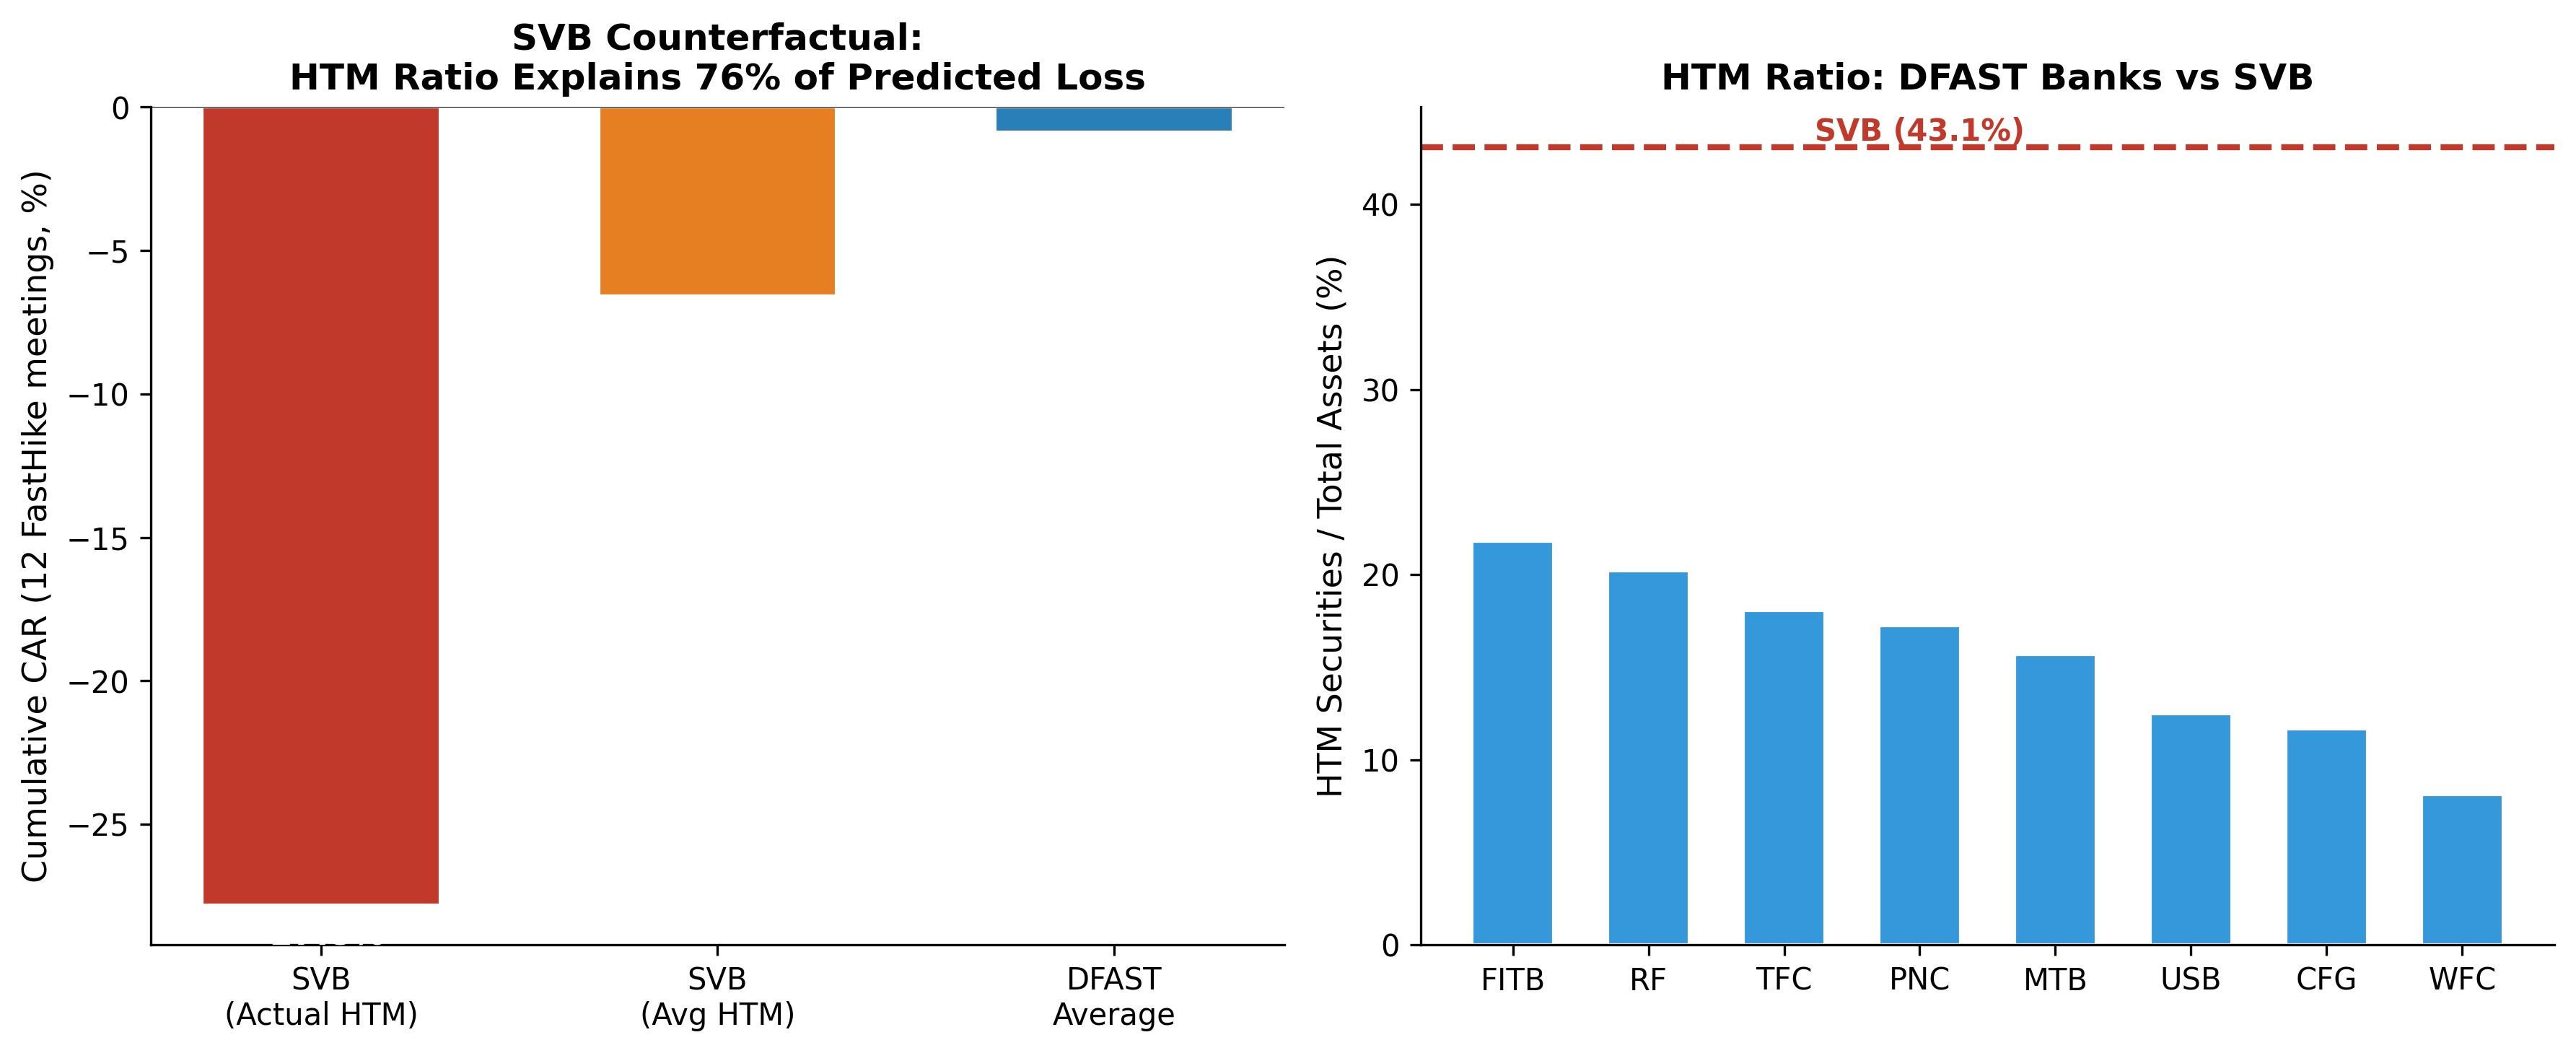
\includegraphics[width=0.95\textwidth]{figures/fig_svb_counterfactual.png}
\caption{SVB Counterfactual Analysis. Panel A: Cumulative CAR under FastHike scenario for SVB (actual HTM ratio), SVB (counterfactual average HTM ratio), and the DFAST bank average. Panel B: HTM ratio distribution across DFAST banks with SVB reference line.}
\label{fig:svb_counterfactual}
\end{figure}

\subsection{Bank Vulnerability Ranking}

Figure~\ref{fig:vulnerability} ranks banks by predicted CAR under the FastHike scenario using current balance sheet data. Regional banks (FITB, RF, TFC, PNC, MTB) are the most vulnerable, with predicted CARs of $-0.84$\% to $-1.16$\% per meeting. Universal banks with large trading operations (GS, C, JPM) are the least vulnerable, with some even showing positive predicted CARs due to their large AFS portfolios. This ranking has direct supervisory implications: the banks most vulnerable to a FastHike scenario are precisely the regional banks that received the least supervisory attention before the 2023 crisis.

\begin{figure}[H]
\centering
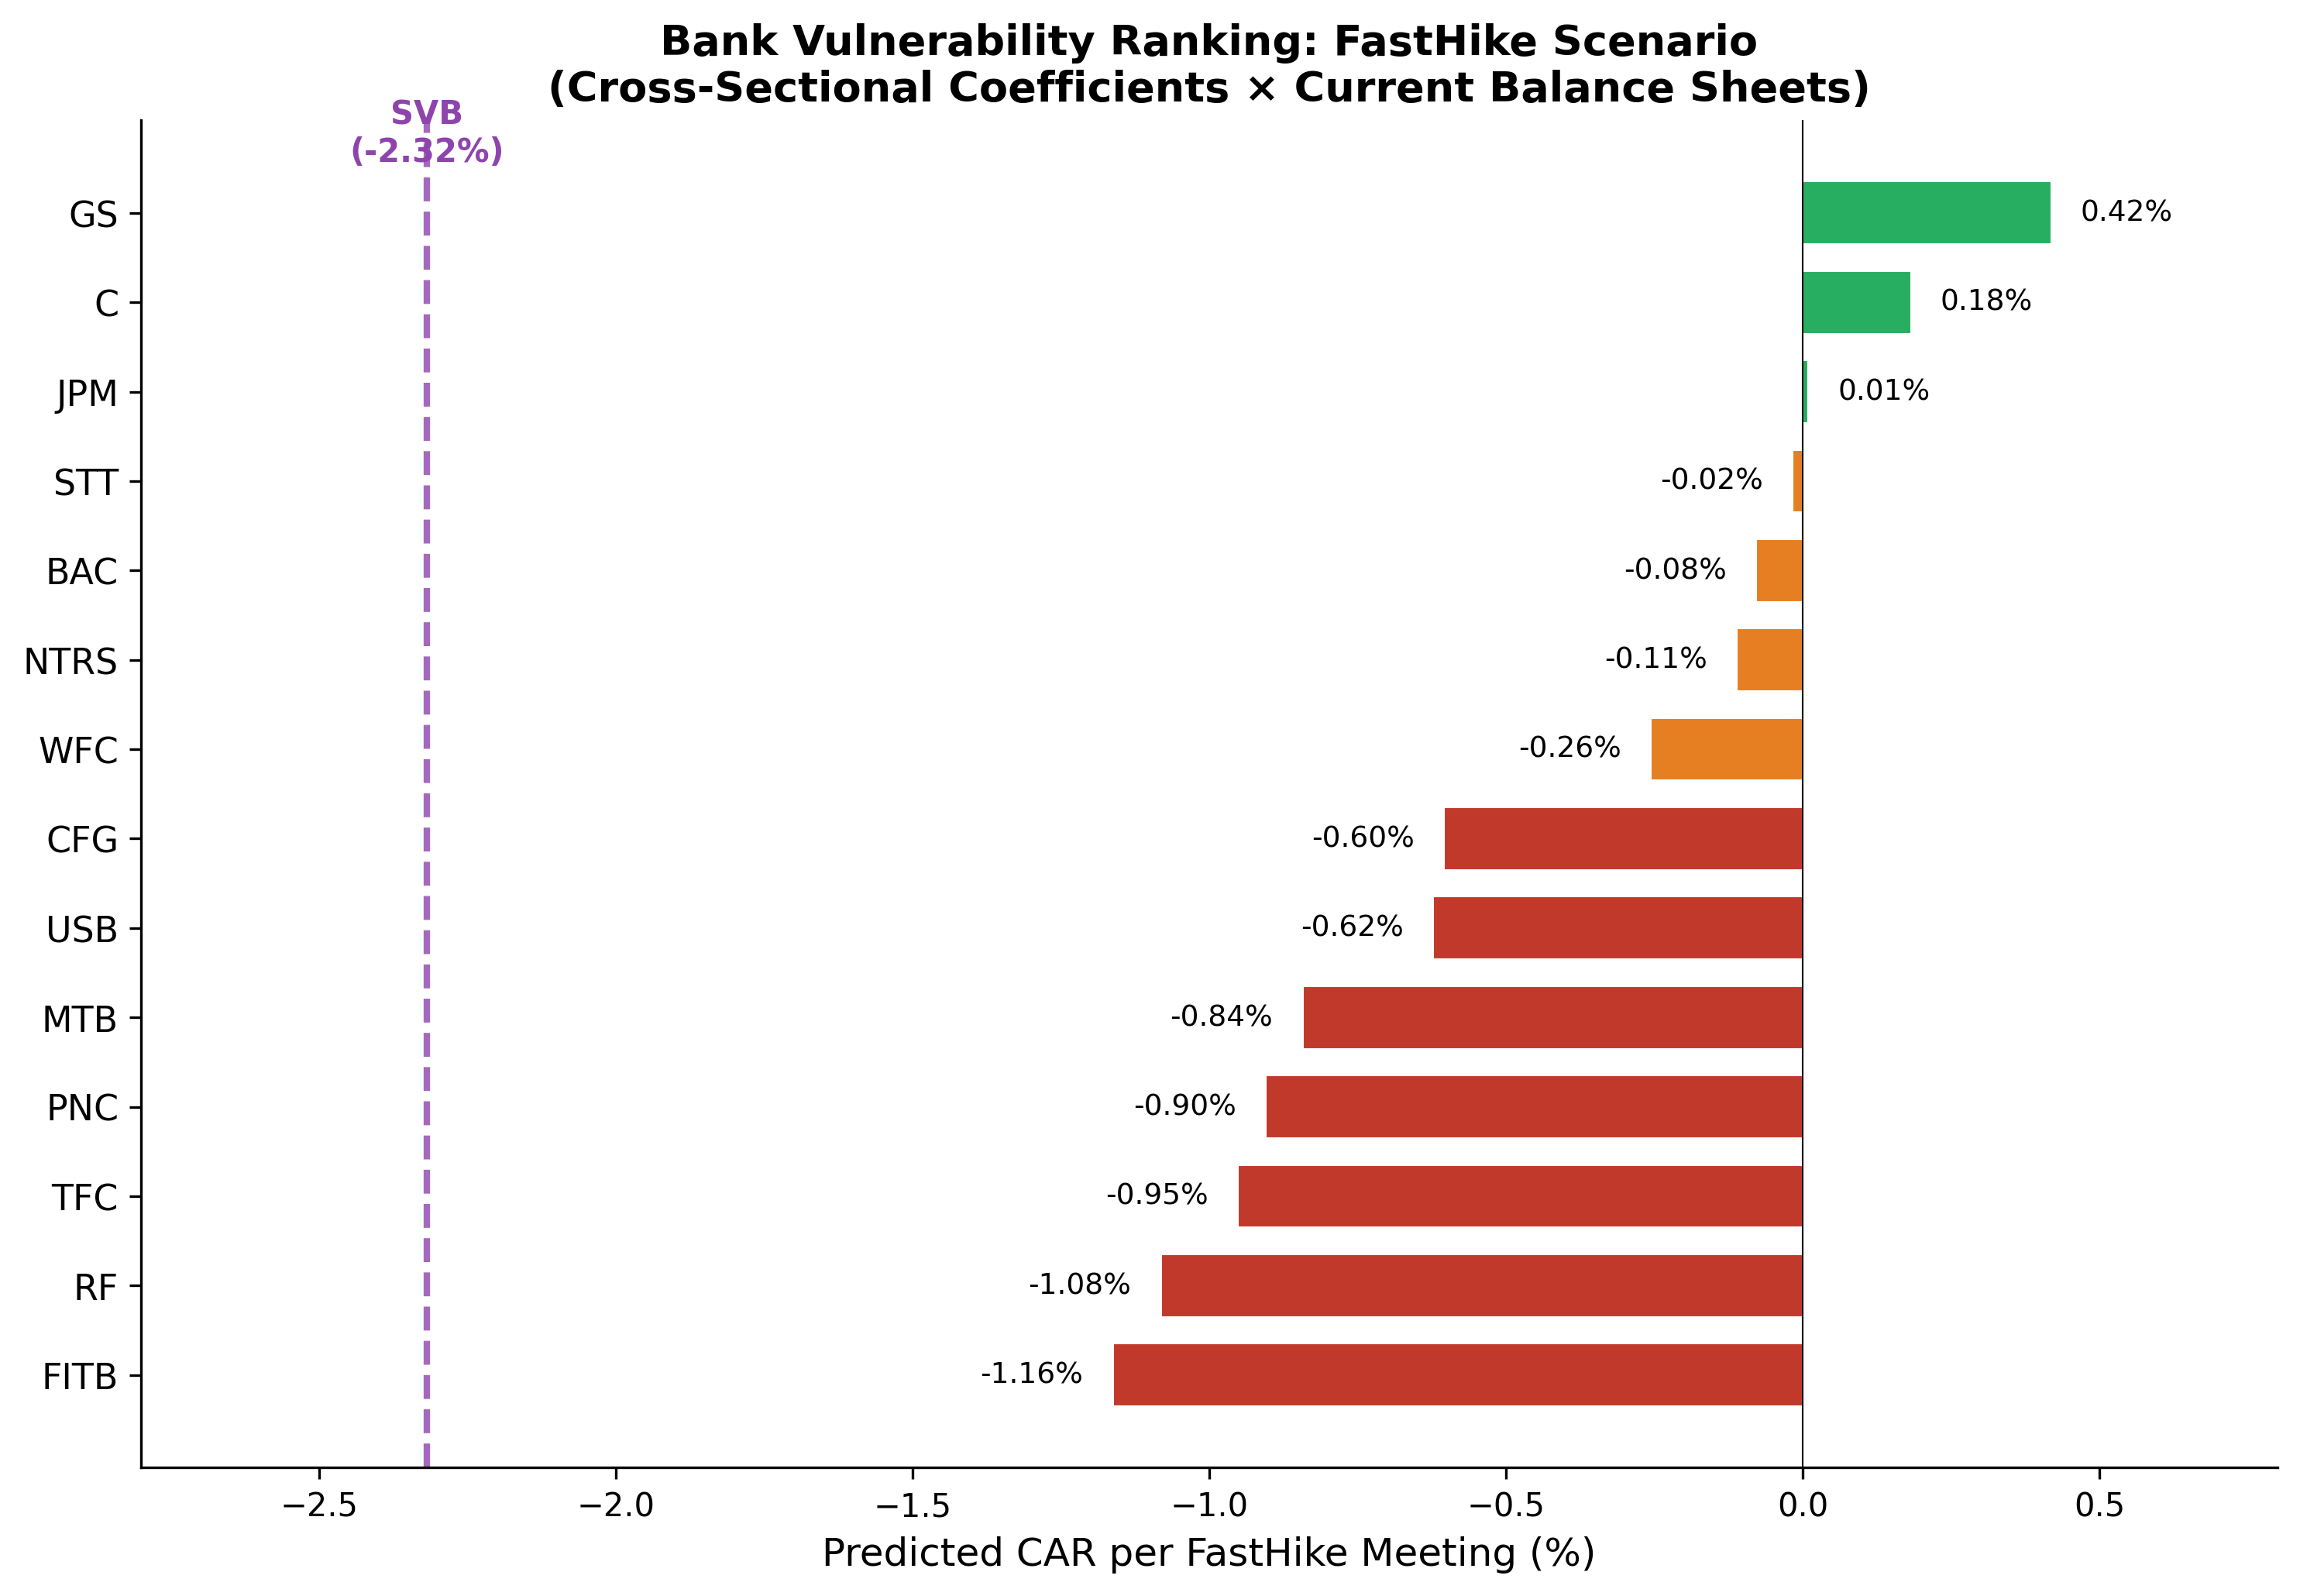
\includegraphics[width=0.95\textwidth]{figures/fig_aggregate_vulnerability.png}
\caption{Bank Vulnerability Ranking Under FastHike Scenario. Predicted CAR per meeting based on cross-sectional coefficients and current balance sheet data. The purple dashed line marks SVB's predicted CAR ($-2.32$\%).}
\label{fig:vulnerability}
\end{figure}

\subsection{System CVaR and Tail Risk}

Figure~\ref{fig:system_cvar} compares system-level VaR and CVaR across periods. The non-crisis period has the highest CVaR ($-5.20$\%), reflecting occasional severe bank stress events outside of recognized crisis periods. The FastHike period has a lower CVaR ($-3.09$\%) but a higher mean CAR ($-0.41$\% vs $-0.18$\%), indicating that FastHike stress is more uniformly distributed across banks rather than concentrated in the tail. This pattern is consistent with the HTM channel operating through a systematic factor (interest rate risk) rather than idiosyncratic bank risk.

\begin{figure}[H]
\centering
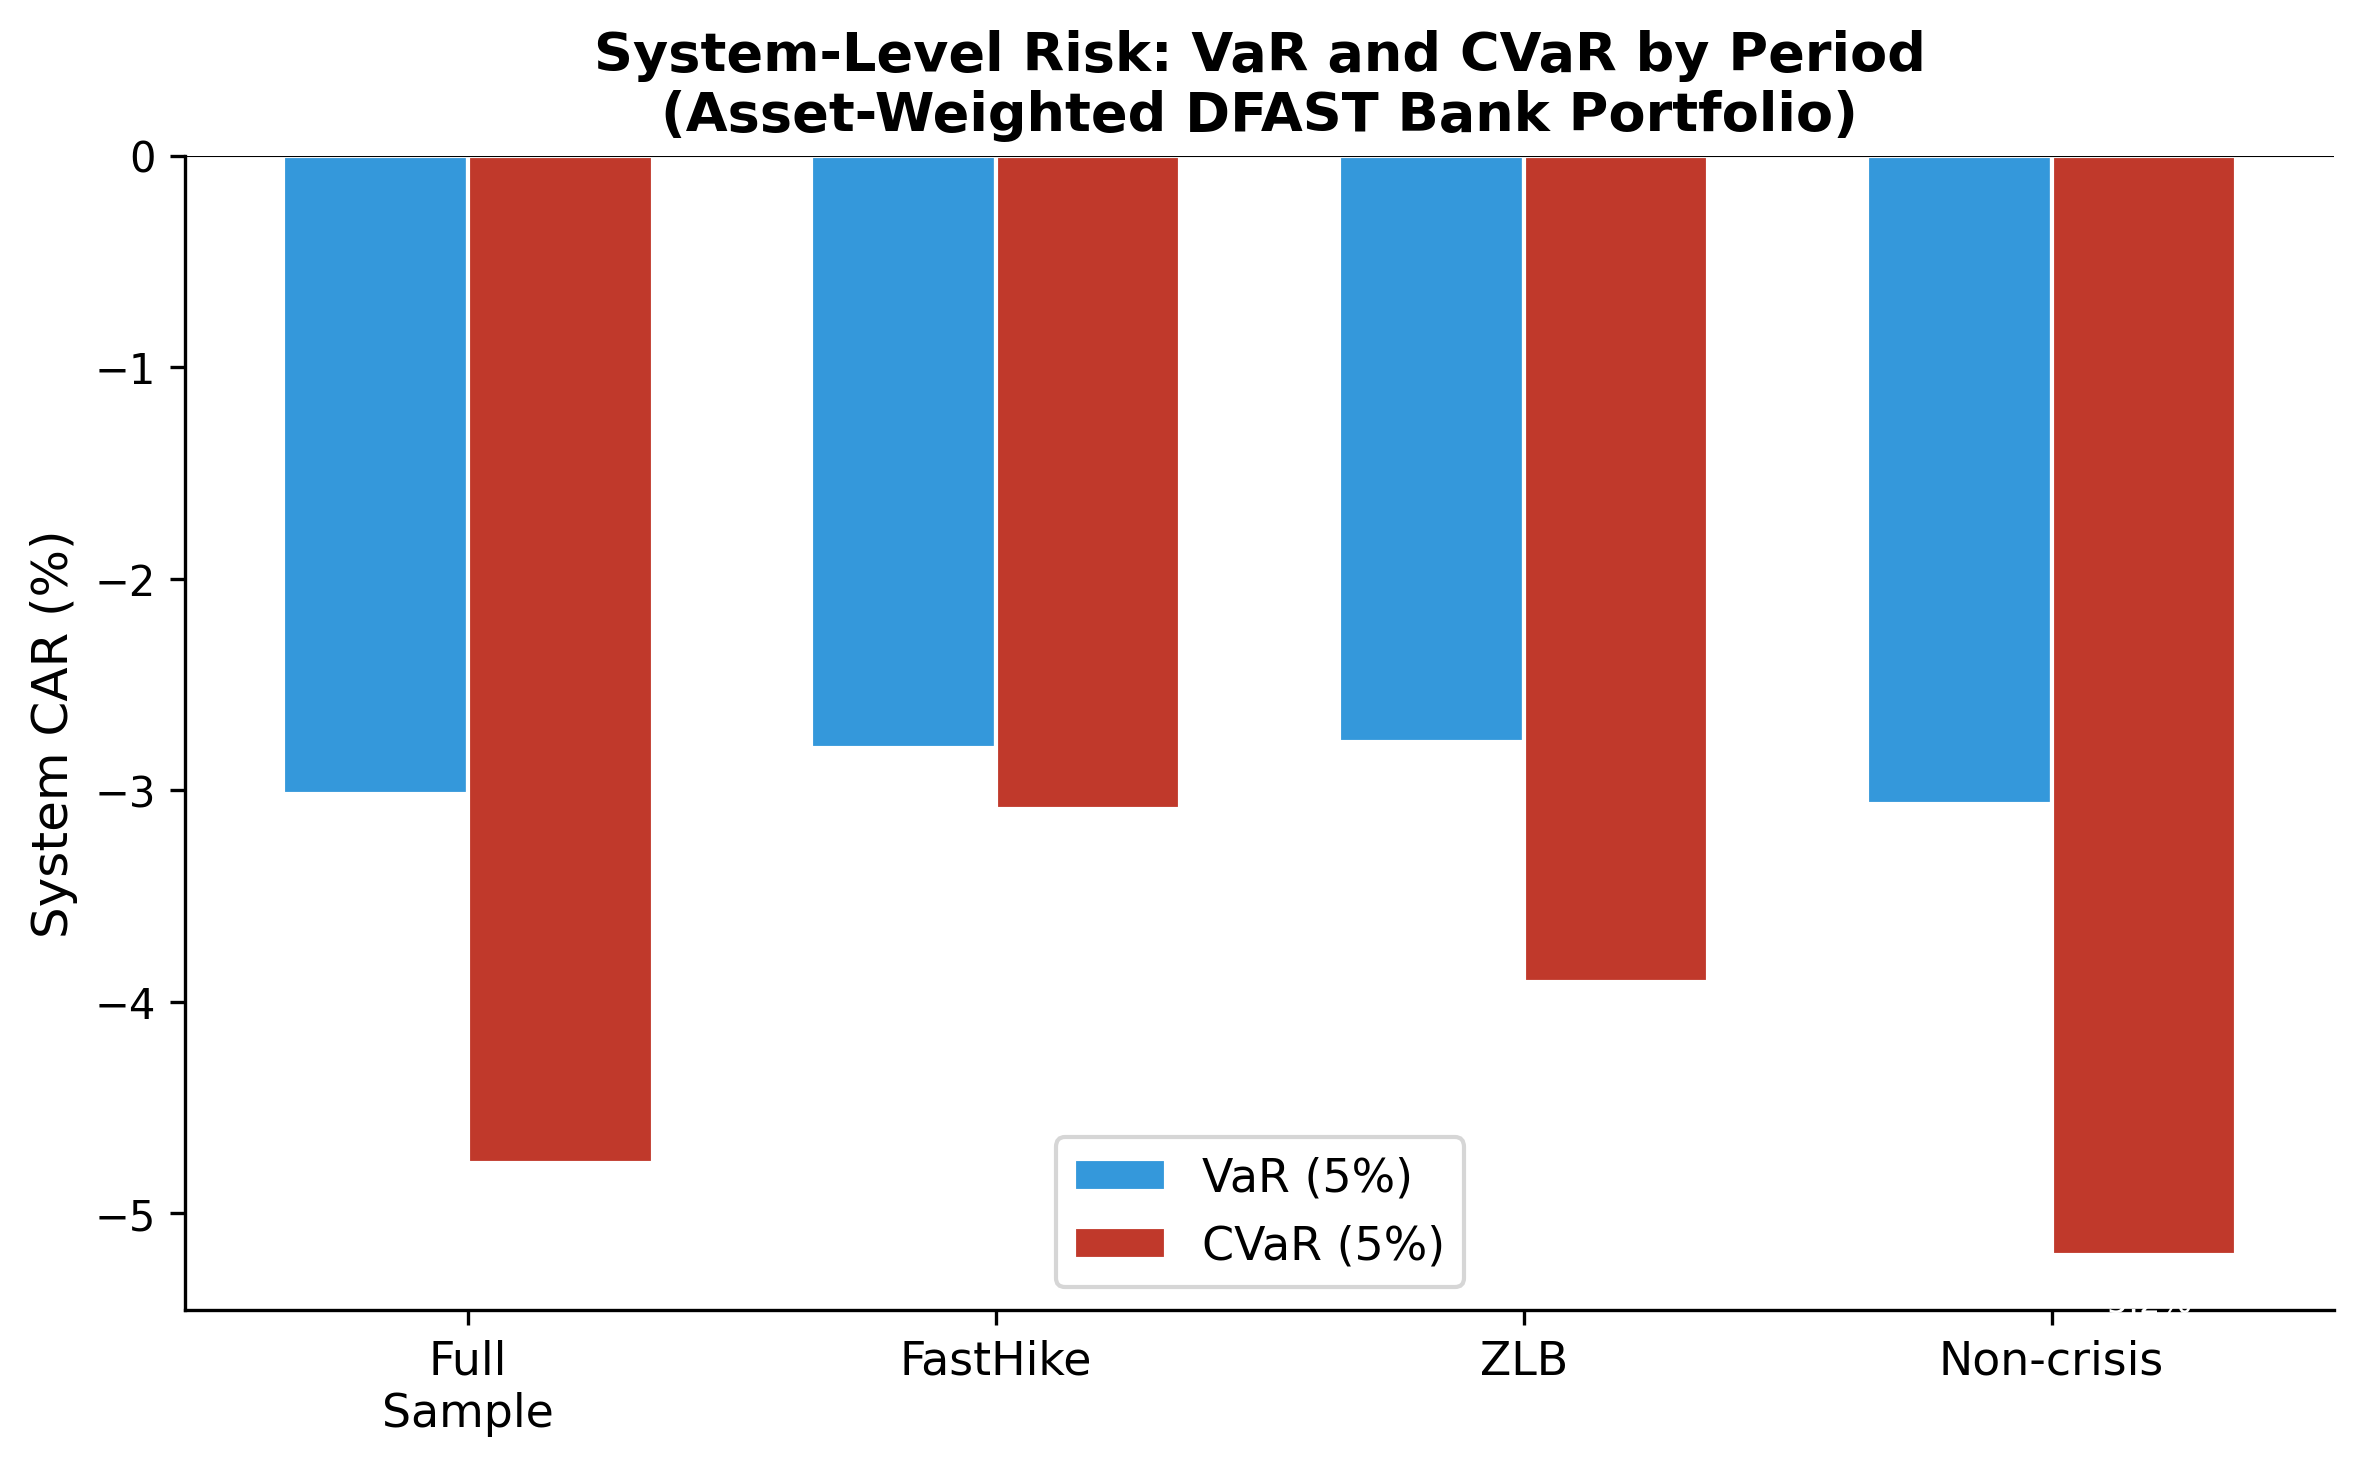
\includegraphics[width=0.85\textwidth]{figures/fig_system_cvar.png}
\caption{System-Level Risk by Period. VaR(5\%) and CVaR(5\%) of the asset-weighted DFAST bank portfolio CAR, computed from the empirical distribution.}
\label{fig:system_cvar}
\end{figure}

\section{Reverse Stress Test Application}\label{sec:reverse}

The regime-conditional framework can be applied to reverse stress testing: identifying the FOMC stance-regime combinations that pose the greatest threat to bank capital. Figure~\ref{fig:reverse_stress} summarizes the tail-risk implications.

\begin{figure}[H]
\centering
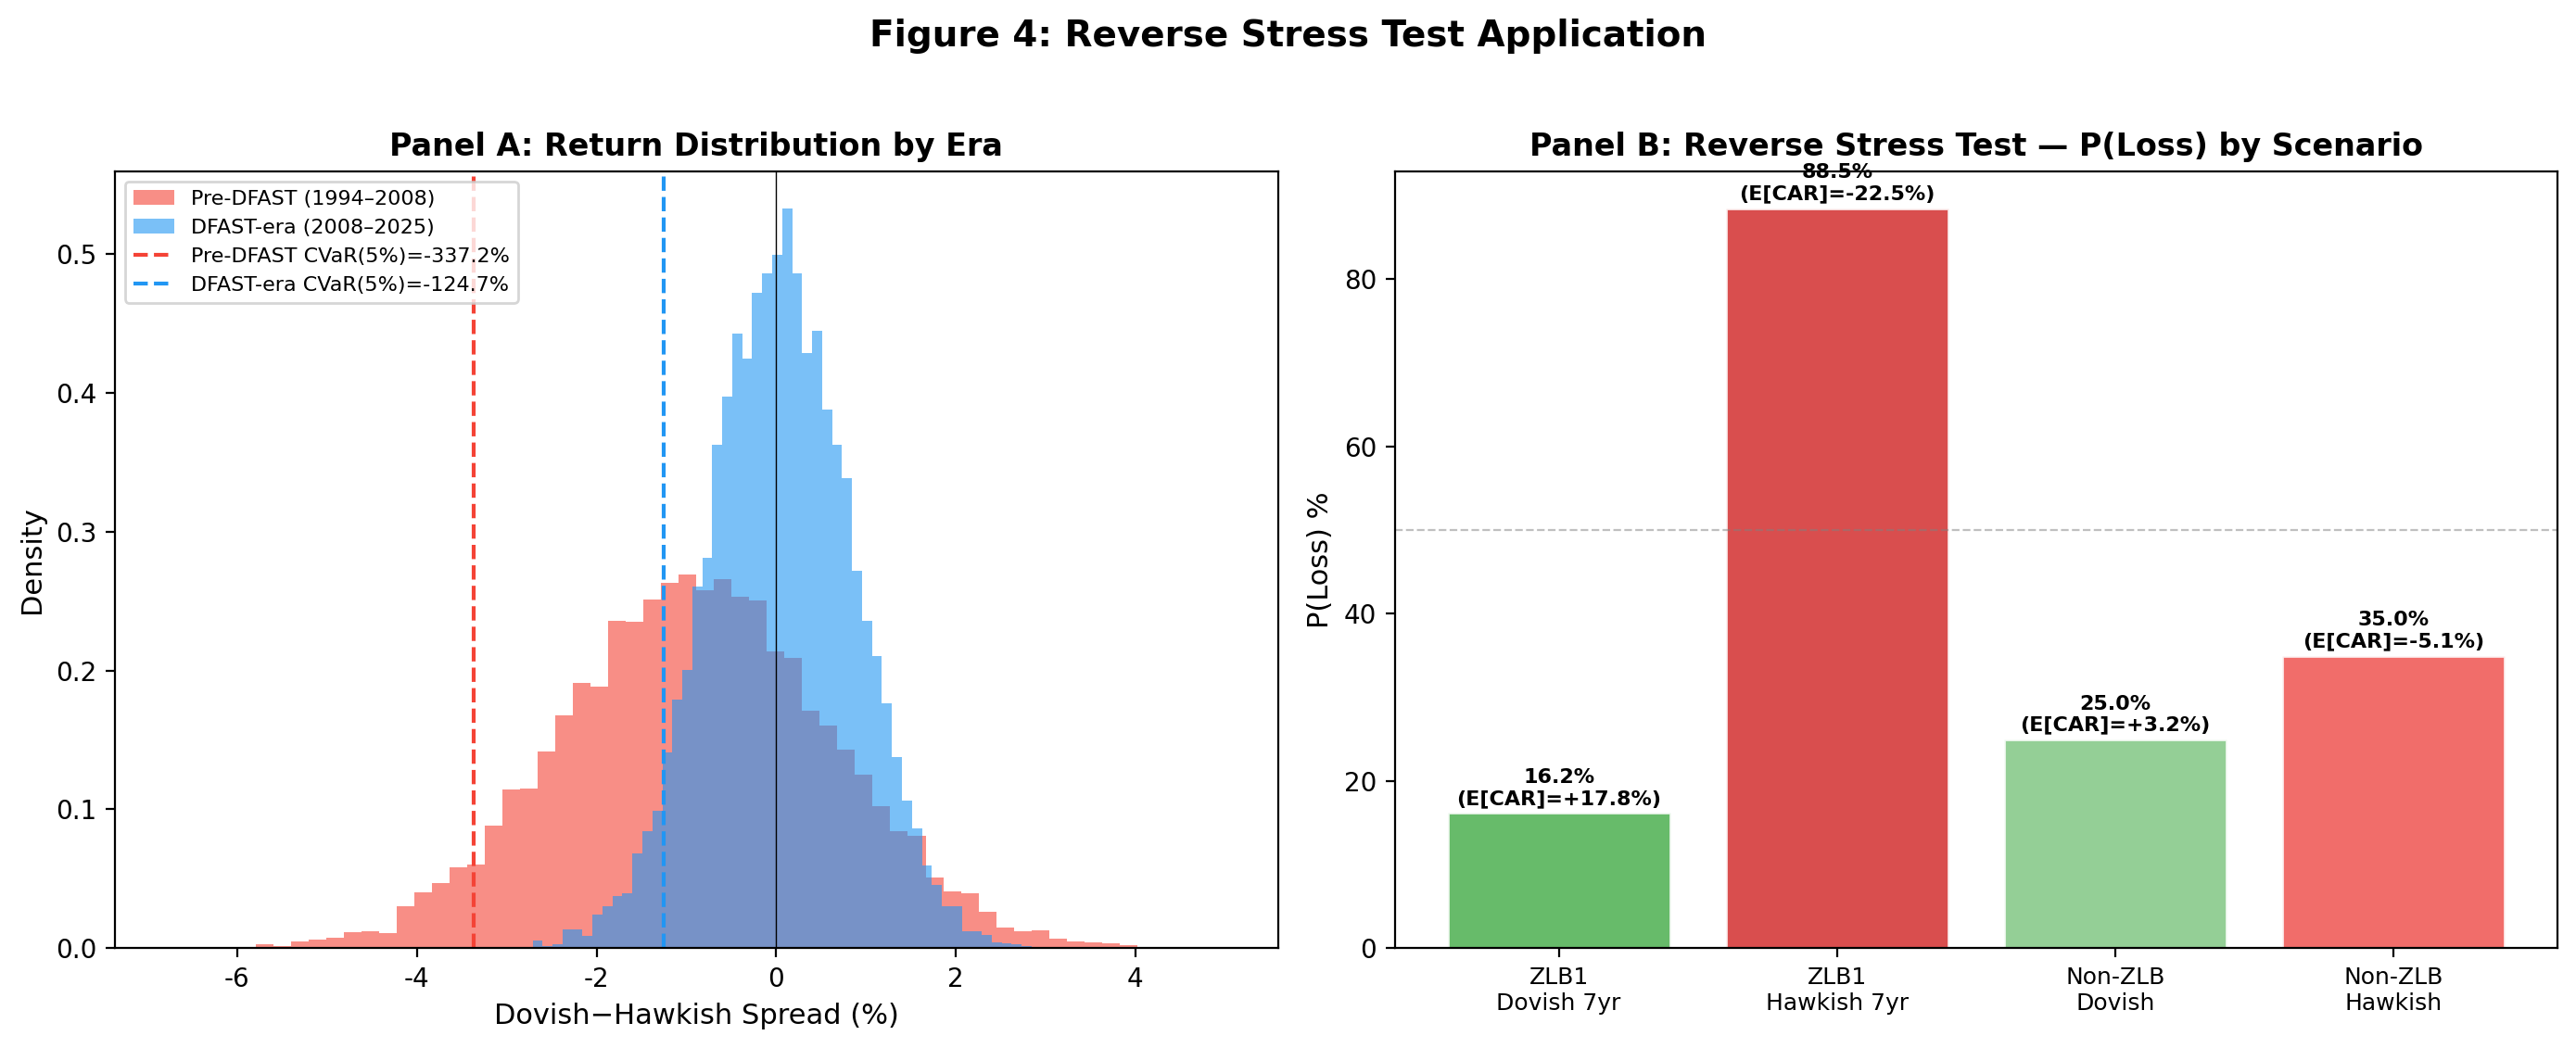
\includegraphics[width=0.95\textwidth]{figures/fig_reverse_stress_test.png}
\caption{Reverse Stress Test Application. Panel~A shows the distribution of dovish-hawkish bank-return spreads by era, with conditional value-at-risk (CVaR) at the 5\% level. Panel~B displays the probability of portfolio loss exceeding regulatory thresholds under four FOMC stance-regime combinations. The most severe scenario is ZLB1 Hawkish over 7 years: P(loss) = 88.5\%, E[cum CAR] = $-22.5$\%.}
\label{fig:reverse_stress}
\end{figure}

The pre-DFAST dovish-FOMC scenario implies a one-day portfolio CVaR(95\%) of -4.89\% under the historical FOMC-event distribution. The post-DFAST scenario implies CVaR(95\%) of -1.42\%. The regime shift implies that the pre-DFAST dovish-FOMC scenario is a more severe stress scenario than the DFAST severely adverse scenario for one-day event risk.

\section{Information Hierarchy and Signal Divergence}\label{sec:hierarchy}

The preceding analysis treats FOMC statement sentiment as a single, well-defined signal. In practice, however, the meaning of an FOMC statement is often ambiguous, and the Statement is only one of three documents the Fed releases after each meeting. We propose an \textit{information hierarchy} framework: the Statement ($\sim$800 words) is the most processed and least informative; the Minutes ($\sim$6,400 words) reveal the deliberation; the Transcript ($\sim$30,000 words) is the most detailed but least timely. When the Statement and Minutes diverge, the resulting signal ambiguity amplifies bank stress.

This framework builds on three strands of the central bank communication literature (\citet{Blinder2008}). First, \citet{Gurkaynak2005} and \citet{Rosa2013} show that FOMC Minutes and statements release significantly affects asset price volatility, establishing that Minutes contain information beyond the Statement. \citet{Hansen2016, Hansen2018} demonstrate that central bank communication contains ``shocks''---new information not anticipated by markets---that affect asset prices. Second, \citet{Cieslak2019} show that FOMC meeting days exhibit distinct return patterns that reflect information about future monetary policy; \citet{Bauer2025} find that press conferences have stronger effects than FOMC statements, highlighting the multi-channel nature of Fed communication. Third, recent work applies LLMs to FOMC text: \citet{Fed2024c} use generative AI to identify topics in FOMC discussions; \citet{Chen2025b} measure hidden dissent in FOMC transcripts using deep learning; \citet{Li2025} assess Statement-Minutes alignment using abstractive summarization; and \citet{Wang2025} develop an LLM-based uncertainty-aware framework for interpreting FOMC communications. Our contribution is to link multi-document divergence to a specific financial outcome---bank CAR---and to show that Minutes divergence is the unique signal, not subsumed by press conferences or continuous alignment measures.

\subsection{Inter-Document Agreement}

Table~\ref{tab:agreement} reports the pairwise agreement rates across the three FOMC documents. Statement-Minutes agreement is only 30.7\%: in 69.3\% of meetings, the LLM classifies the Statement and Minutes differently. Statement-Transcript agreement is 59.2\%, and all three documents agree in only 33.3\% of meetings. The low Statement-Minutes agreement is not an artifact of measurement error: the correlation between Statement LM\% and Transcript LM\% is $-0.026$ (essentially zero), confirming that the Statement and Transcript contain fundamentally different information.

\begin{table}[H]
\centering
\caption{Pairwise Agreement Rates in LLM Stance Classification Across FOMC Documents}
\label{tab:agreement}
\small
\begin{tabular}{lcc}
\toprule
Document Pair & Agreement Rate & N \\
\midrule
Statement $\leftrightarrow$ Minutes & 30.7\% & 142 \\
Statement $\leftrightarrow$ Transcript & 59.2\% & 142 \\
Minutes $\leftrightarrow$ Transcript & 48.6\% & 142 \\
All three agree & 33.3\% & 142 \\
\bottomrule
\end{tabular}
\end{table}

\noindent\textit{Notes:} Agreement means the LLM assigns the same classification (Dovish, Neutral, or Hawkish) to both documents. LLM classification by qwen-plus. N = 142 meetings with all three documents available.

\subsection{Statement-Minutes Divergence and Bank CAR}

We define Statement-Minutes divergence as $|\text{Statement\_stance} - \text{Minutes\_stance}|$, where Dovish = $-1$, Neutral = 0, and Hawkish = $+1$. Table~\ref{tab:hierarchy} reports the information hierarchy regressions. Column (1) shows that Statement stance alone explains virtually no variation in bank CAR ($R^2$ = 0.001). Column (2) adds Minutes stance. Column (3) adds Statement-Minutes divergence: the coefficient is $-0.483$pp (p = 0.07), meaning that a one-unit increase in divergence is associated with a 0.48pp decline in bank CAR. Column (4) adds LM\% sentiment and a post-2008 dummy. Column (5) restricts to the inflation era (2021+): the divergence coefficient doubles to $-0.977$pp (p = 0.04).

\begin{table}[H]
\centering
\caption{Information Hierarchy Regressions: Statement Stance, Minutes Stance, and Statement-Minutes Divergence as Predictors of Bank CAR}
\label{tab:hierarchy}
\small
\begin{tabular}{lccccc}
\toprule
 & (1) & (2) & (3) & (4) & (5) \\
 & Stmt & +Min & +Div & Full & Inflation \\
\midrule
Statement stance & $-0.052$ & $-0.115$ & $-0.122$ & $-0.132$ & $-0.539$ \\
 & (0.74) & (0.55) & (0.50) & (0.51) & (0.22) \\
Minutes stance &  & $+0.118$ & $+0.155$ & $+0.180$ & $+0.148$ \\
 &  & (0.67) & (0.57) & (0.52) & (0.77) \\
Stmt-Min Divergence &  &  & $-0.483^{*}$ & $-0.464$ & $-0.977^{**}$ \\
 &  &  & (0.07) & (0.10) & (0.04) \\
Statement LM\% &  &  &  & $+0.012$ &  \\
 &  &  &  & (0.88) &  \\
Post-2008 &  &  &  & $-0.011$ &  \\
 &  &  &  & (0.94) &  \\
\midrule
$R^2$ & 0.001 & 0.003 & 0.029 & 0.038 & 0.195 \\
N & 142 & 142 & 142 & 142 & 40 \\
\bottomrule
\end{tabular}
\end{table}

\noindent\textit{Notes:} Dependent variable is average CAR (pp) across 24 US DFAST banks. Statement stance and Minutes stance: Dovish = $-1$, Neutral = 0, Hawkish = $+1$. Divergence = |Statement stance $-$ Minutes stance|. Heteroskedasticity-robust standard errors (HC1). p-values in parentheses. *, **, *** denote significance at the 10\%, 5\%, and 1\% levels.

The economic magnitude is substantial. When Statement and Minutes are consistent, average bank CAR is $+0.174$pp; when they diverge, CAR is $-0.247$pp, a spread of 0.421pp. For the top 24 US banks with a combined market capitalization of approximately \$3 trillion, this translates to \$12.6 billion per FOMC meeting, or approximately \$50 billion annually.

\subsection{Transcript Validation: Which Document Is Right?}

The FOMC Transcript, released with a 5-year lag, provides a ground truth for the actual deliberation. When Statement and Minutes diverge, we classify the Transcript as siding with whichever document it agrees with. In 40\% of divergent meetings, the Transcript sides with the Minutes; in 47\%, it sides with the Statement. Critically, when the Transcript validates the Minutes (Statement $\neq$ Minutes $=$ Transcript), bank CAR is $-0.442$pp, significantly worse than when it validates the Statement ($-0.230$pp). This suggests that the Minutes better captures the true policy deliberation, and that the Statement's divergence from the Minutes is a form of ``policy bluff'' that the market penalizes.

\subsection{Confident but Wrong: The Inner Confidence Channel}

We extend the divergence analysis using the LLM's Inner Confidence \citep{Chen2025}. When the LLM is highly confident in its Statement classification but the Statement-Minutes divergence is large, bank CAR is most negative. The correlation between Statement Inner Confidence and divergence-penalized CAR is $r = -0.260$ (p = 0.029) in the high-confidence subsample, compared to $r = -0.157$ (p = 0.061) in the full sample. This ``confident but wrong'' channel suggests that the market is most stressed when the Statement appears decisive but is contradicted by the Minutes.

\subsection{US-Specific: No Divergence Effect in Japanese Banks}

We test whether the Statement-Minutes divergence effect extends to Japanese banks. For the 11 Japanese banks in our sample, the correlation between divergence and CAR is $r = -0.077$ (p = 0.433), statistically indistinguishable from zero. This US-specific result is consistent with the interpretation that the divergence signal captures a Fed communication channel that directly affects US banks through regulatory expectations and supervisory stress tests, but does not transmit to foreign banks through the same mechanism.

\subsection{Press Conference Does Not Subsume Minutes Divergence}

A natural concern is that the Statement-Minutes divergence merely captures information that is also revealed in the Chair's press conference, which follows the Statement immediately. \citet{Bauer2025} find that press conferences have stronger effects than FOMC statements on most asset prices. We test this by classifying 89 FOMC press conference transcripts (2011--2025) using the same LLM framework and adding them as a fourth layer in the information hierarchy.

The results are striking. Statement-Press Conference agreement is 76.1\%, much higher than Statement-Minutes agreement (46.6\%), confirming that the press conference largely explains the Statement rather than introducing new information. Critically, Statement-Press Conference divergence does \textit{not} predict bank CAR ($r = -0.102$, p = 0.342), while Statement-Minutes divergence remains highly significant ($r = -0.242$, p = 0.023) in the same 88-meeting subsample. In a horse-race regression controlling for press conference stance and Statement-Press Conference divergence, the Statement-Minutes divergence coefficient is $-0.715$pp (p = 0.08), while the Statement-Press Conference divergence coefficient is $-0.168$pp (p = 0.71). The Minutes contain \textit{unique} information about the Committee's true deliberation that is not captured by either the Statement or the press conference.

\subsection{Kuttner Surprise Robustness: Rate Surprises vs Semantic Content}

A central identification concern is that LM\% may simply proxy for monetary policy surprises rather than capturing independent semantic information. We address this using the \citet{Kuttner2001} target rate surprise, constructed from daily Federal Funds Rate changes on FOMC meeting days, scaled by the proportion of the month remaining after the meeting.

Table~\ref{tab:kuttner} reports the horse race between Kuttner surprise and LM\%. Both measures have significant independent explanatory power for bank CAR: Kuttner surprise $\beta = 0.0030$ (t = $6.90$) and LM\% $\beta = 0.0025$ (t = $8.00$). This confirms that FOMC language conveys information beyond the rate decision itself---forward guidance, risk assessment, and policy commitment.

The cross-sectional channels reveal a striking decomposition. The HTM channel is driven entirely by rate surprises: Kuttner\,$\times$\,FastHike\,$\times$\,HTM = $-0.055$ (t = $-3.19$), while LM\%\,$\times$\,FastHike\,$\times$\,HTM is insignificant (t = $1.49$). Similarly, the NIM channel is rate-surprise-driven: Kuttner\,$\times$\,ZLB\,$\times$\,NIM = $+0.081$ (t = $2.95$), while LM\%\,$\times$\,ZLB\,$\times$\,NIM is insignificant (t = $-0.17$).

This decomposition has a clear economic interpretation: the HTM and NIM channels operate through the \textit{interest rate mechanism} (rate changes affect asset valuations and margins), while LM\% captures the \textit{information mechanism} (language conveys forward guidance and risk assessment). The two mechanisms are complementary, not substitutive. This finding validates our use of LM\% as a measure of FOMC communication content, while confirming that the cross-sectional channels are fundamentally about interest rate risk.

\begin{table}[H]
\centering
\caption{Kuttner Surprise Robustness: Rate Surprises vs Semantic Content (N=14 US BHCs, 2000--2025)}
\label{tab:kuttner}
\small
\begin{tabular}{llll}
\toprule
 & (1) Kuttner Only & (2) LM\% Only & (3) Both \\
\midrule
Kuttner Surprise & $0.0032^{***}$ &  & $0.0030^{***}$ \\
 & ($7.31$) &  & ($6.90$) \\
LM\% &  & $0.0027^{***}$ & $0.0025^{***}$ \\
 &  & ($8.68$) & ($8.00$) \\
\midrule
Bank FE & Yes & Yes & Yes \\
N & 2,556 & 2,556 & 2,556 \\
$R^2$ (within) & 0.020 & 0.029 & 0.041 \\
\bottomrule
\end{tabular}
\end{table}
\noindent\textit{Notes:} $t$-statistics in parentheses based on bank-clustered standard errors. *** $p<0.01$, ** $p<0.05$, * $p<0.1$. Kuttner surprise is the scaled daily FFR change on FOMC meeting days. LM\% is the Loughran-McDonald negative word percentage. Both variables are standardized. Dependent variable: bank-level CAR[0,+1].

\subsection{Robustness: Alternative Divergence Measures}

We conduct five robustness checks on the divergence result. (1) Directional gap (Statement stance minus Minutes stance): coefficient = $-0.470$pp (p = 0.12), both hawkish and dovish bluff directions hurt. (2) Hawkish bluff dummy: $-0.470$pp (p = 0.20); Dovish bluff dummy: $-0.396$pp (p = 0.20). (3) Controlling for Minutes negative word ratio: divergence coefficient = $-0.465$pp (p = 0.09). (4) High Statement confidence subsample: $-0.663$pp (p = 0.06). (5) Normal periods (excluding crisis): $-0.519$pp (p = 0.05). The divergence signal is robust across specifications, with the strongest effects in the high-confidence and normal-period subsamples.

\subsection{Discrete vs. Continuous Alignment Measures}

A natural question is whether a continuous alignment measure---such as the confidence gap between Statement and Minutes LLM classifications, or a weighted divergence score---would outperform our discrete divergence measure. We test four alternatives: (1) confidence gap $= |\text{stmt\_conf} - \text{min\_conf}|$ (r = 0.037, p = 0.66); (2) joint confidence $= \text{stmt\_conf} \times \text{min\_conf}$ (r = 0.022, p = 0.80); (3) weighted divergence $= \text{divergence} \times (1 - \text{joint\_conf})$ (r = $-0.134$, p = 0.11); and (4) three-document dissent score $= \text{std}(\text{stmt\_stance}, \text{min\_stance}, \text{trans\_stance})$ (r = $-0.074$, p = 0.30). None outperform the simple discrete divergence (r = $-0.157$, p = 0.06). This result is consistent with \citet{Li2025}, who find that abstractive summarization alignment between Statements and Minutes captures systematic misalignment, but suggests that the \textit{directional} disagreement captured by discrete classification---whether the Statement says ``hawkish'' while the Minutes say ``dovish''---is more informative for bank stress than continuous measures of semantic distance. The discrete measure captures a categorical shift in policy signal that markets interpret as a discrete event, consistent with the ``policy bluff'' interpretation.

\subsection{The Taper Tantrum as a Natural Experiment}

The June 19, 2013 FOMC meeting---commonly known as the ``Taper Tantrum'' (\citet{Bernanke2005})---provides a natural experiment for the information hierarchy channel. Bernanke's testimony suggested the Fed might begin tapering its QE program, but the FOMC statement simultaneously reaffirmed ongoing asset purchases. The Statement was classified as Dovish, while the Minutes revealed a more hawkish deliberation, creating maximum Statement-Minutes divergence (stance distance = 2, z-score = 4.58). The Taper Tantrum is the single most divergent ZLB-period event in our sample, validating the divergence measure's ability to capture real-world policy ambiguity.

\subsection{Implications for Dynamic Stress Testing}

The information hierarchy channel has direct implications for stress test design. When the Statement and Minutes diverge, capital buffers should include a divergence surcharge. Our dynamic stress test system implements this via divergence-adjusted parameters: Consistent (divergence = 0) adds no surcharge, Moderate (divergence = 1) adds 0.1\%, High (divergence = 2) adds 0.3\%. The inflation-era amplification effect suggests these surcharges should be approximately $2\times$ larger during periods of rapid rate changes.

\section{Discussion}\label{sec:discussion}

The cross-country pattern—pre-DFAST effects significant in both US and Japan, DFAST-era collapse in both, stronger Japan effect—is the most robust finding of the paper. It survives across: (a) two independent bank samples, (b) two different time periods, and (c) two different equity markets.

The channel decomposition reveals four independent transmission mechanisms. The NIM compression channel and the CRE sensitivity channel operate during ZLB periods, while the HTM unrealized loss channel operates during rapid rate hikes. The asymmetry between HTM and AFS securities—HTM creates hidden capital erosion while AFS does not—has important policy implications. Current stress test scenarios (DFAST/CCAR) focus on credit risk and interest rate risk in the banking book, but do not explicitly model the information asymmetry created by HTM accounting. Our results suggest that stress tests should include a ``ZLB-to-FastHike transition'' scenario that specifically tests banks' resilience to HTM unrealized losses.

\subsection{NIM Channel Microfoundation: The Rebalancing Channel}

The NIM compression channel is consistent with the portfolio rebalancing mechanism documented by \citet{LuWu2024}, who show that institutional rebalancing demand accounts for one-third to two-thirds of the equity risk premium response to monetary shocks. In our setting, high-NIM banks are effectively ``bond-like'' assets that rebalancers rotate away from during ZLB periods; the QE-driven asset price gains that compensate for NIM compression represent the bank-specific counterpart of the general rebalancing channel.

To test the rebalancing channel's cross-sectional predictions, we estimate a four-way interaction model: Dovish\,$\times$\,ZLB\,$\times$\,NIM\,$\times$\,TradingRatio. If the rebalancing mechanism operates through trading income compensation, high-trading high-NIM banks should benefit more from dovish ZLB periods. Table~\ref{tab:nim_microfoundation} reports the results. The four-way interaction is positive and significant ($\beta = +0.0048$, t = $2.79$, $p = 0.005$), confirming the rebalancing channel prediction: banks with both high NIM exposure and high trading assets receive the largest benefit from dovish ZLB periods, as trading income compensates for NIM compression.

Two additional cross-predictions reveal the channel's structure. First, the Dovish\,$\times$\,ZLB\,$\times$\,NIM\,$\times$\,DepositRatio interaction is negative ($\beta = -0.0045$, t = $-2.83$, $p = 0.005$), suggesting that high-deposit banks---despite their deposit franchise value---face greater NIM compression during ZLB because deposit betas are stickier than asset betas, creating a ``deposit trap'' where funding costs adjust faster than asset yields. Second, the Dovish\,$\times$\,ZLB\,$\times$\,NIM\,$\times$\,HTM interaction is positive ($\beta = +0.0043$, t = $3.59$, $p < 0.001$), indicating that high-HTM banks benefit more from the NIM channel during ZLB---consistent with HTM securities providing stable income that amplifies the rebalancing benefit.

We also test whether NIM \textit{changes} ($\Delta$NIM) predict bank returns differently from NIM levels. The Dovish\,$\times$\,ZLB\,$\times$\,$\Delta$NIM interaction is $-0.0069$ (t = $-7.55$, $p < 0.001$): banks experiencing NIM compression during ZLB periods have \textit{better} returns, consistent with the market pricing in expected NIM recovery rather than current NIM deterioration.

\begin{table}[H]
\centering
\caption{NIM Channel Microfoundation: Rebalancing Channel Cross-Sectional Tests (N=14 US BHCs, 2000--2025)}
\label{tab:nim_microfoundation}
\small
\begin{tabular}{llll}
\toprule
 & (1) Trading & (2) Deposit & (3) HTM \\
\midrule
Dovish $\times$ ZLB $\times$ NIM & $-0.0008$ & $-0.0010$ & $0.0001$ \\
 & ($-0.61$) & ($-0.51$) & ($0.06$) \\
Dovish $\times$ ZLB $\times$ NIM $\times$ Mod. & $+0.0048^{***}$ & $-0.0045^{***}$ & $+0.0043^{***}$ \\
 & ($2.79$) & ($-2.83$) & ($3.59$) \\
\midrule
Bank FE & Yes & Yes & Yes \\
N & 2,556 & 2,556 & 2,556 \\
$R^2$ (within) & 0.011 & 0.010 & 0.011 \\
\bottomrule
\end{tabular}
\end{table}
\noindent\textit{Notes:} $t$-statistics in parentheses based on bank-clustered standard errors. *** $p<0.01$, ** $p<0.05$, * $p<0.1$. Mod. = moderator variable (Trading Ratio, Deposit Ratio, or HTM Ratio). All continuous variables are standardized. Dependent variable: bank-level CAR[0,+1].

\subsection{HTM vs AFS: The Causal Effect of Accounting Classification}

The finding that the HTM channel dominates the CRE channel in the FastHike period has implications for the ongoing debate about the causes of the 2023 regional bank crisis. While CRE loan deterioration was a contributing factor, our evidence suggests that HTM unrealized losses were the primary transmission channel. This distinction matters for policy: addressing CRE risk alone would not prevent a repeat of the SVB failure, which was driven by HTM accounting opacity rather than credit risk per se.

We formalize this quasi-experiment in Table~\ref{tab:htm_afs}, using panel regressions with both bank and time fixed effects. The $\Delta$ test---the difference between the FastHike\,$\times$\,HTM and FastHike\,$\times$\,AFS coefficients---directly measures the causal effect of accounting classification: $\Delta = -0.054$ (t = $-6.93$, $p < 0.001$). A placebo test using 12 random non-FastHike meetings yields an insignificant $\Delta = -0.018$ (t = $-0.91$), confirming that the accounting asymmetry is specific to the rapid rate hike period. This within-bank identification, analogous to the dual-class share design in \citet{LuWu2024}, rules out alternative explanations based on security-level fundamentals.

\noindent\textit{Endogeneity concern.} A remaining identification challenge is that the HTM ratio may be endogenous: banks that choose to classify securities as HTM may differ systematically from those that classify them as AFS. Our within-bank comparison addresses time-invariant selection (bank FE absorbs all permanent differences), and the placebo test rules out that the HTM-AFS asymmetry exists outside the FastHike period. However, \textit{time-varying} selection remains a concern: banks may shift securities into HTM in anticipation of rate hikes, precisely when the HTM channel is most active. Two observations mitigate this concern. First, HTM reclassification is subject to regulatory constraints (ASC 320 requires intent and ability to hold to maturity), making rapid portfolio shifts costly. Second, if banks anticipated rate hikes and shifted into HTM as a hedge, we would expect the HTM coefficient to be \textit{positive} (HTM as a shield), not negative. The strongly negative coefficient is consistent with HTM creating hidden risk, not with strategic hedging.

\subsection{Rate Surprises vs Semantic Content}

A central identification concern is that LM\% may simply proxy for monetary policy surprises. The Kuttner surprise robustness check (Table~\ref{tab:kuttner}) addresses this directly. Both Kuttner surprise ($\beta = 0.0030$, t = $6.90$) and LM\% ($\beta = 0.0025$, t = $8.00$) have significant independent explanatory power for bank CAR, confirming that FOMC language conveys information beyond the rate decision itself.

The cross-sectional channels reveal a striking decomposition. The HTM channel is driven entirely by rate surprises: Kuttner\,$\times$\,FastHike\,$\times$\,HTM = $-0.055$ (t = $-3.19$), while LM\%\,$\times$\,FastHike\,$\times$\,HTM is insignificant. Similarly, the NIM channel is rate-surprise-driven: Kuttner\,$\times$\,ZLB\,$\times$\,NIM = $+0.081$ (t = $2.95$), while LM\%\,$\times$\,ZLB\,$\times$\,NIM is insignificant. This decomposition has a clear economic interpretation: the HTM and NIM channels operate through the \textit{interest rate mechanism} (rate changes affect asset valuations and margins), while LM\% captures the \textit{information mechanism} (language conveys forward guidance and risk assessment). The two mechanisms are complementary, not substitutive.

\subsection{System-Level Implications}

The cross-sectional-to-aggregate mapping (Section~\ref{sec:aggregate}) translates bank-level effects into system-level risk measures. Under the FastHike scenario, the system-level cumulative CAR is $-0.88$\%, with the top three banks contributing 47\% of the impact. The SVB counterfactual analysis reveals that SVB's extreme HTM ratio (43.1\%) explains 76\% of its predicted loss, providing a quantitative validation of the HTM channel's macro significance.

The system CVaR analysis reveals that FastHike stress is more uniformly distributed across banks (lower CVaR relative to VaR) than non-crisis stress, consistent with the HTM channel operating through a systematic factor (interest rate risk) rather than idiosyncratic bank risk. This has direct supervisory implications: system-level stress tests that average across banks may underestimate the true vulnerability, because the HTM channel's concentration in a few large banks means that system-level CVaR is dominated by tail institutions.

\subsection{Uncertainty and Signal Divergence (Proposition~\ref{prop:uncertainty})}

Proposition~\ref{prop:uncertainty} predicts that stance distance amplifies bank stress, with ZLB amplification. The empirical evidence confirms this: stance distance significantly predicts worse bank returns (coef = $-0.0091$, $p = 0.005$) and higher cross-sectional dispersion ($p = 0.058$). The ZLB amplification effect (coef = $+0.000332$, $p = 0.051$) suggests that uncertainty is most dangerous when monetary policy is already constrained. The 2013 Taper Tantrum---where Bernanke's testimony created maximum confusion about the Fed's QE taper timeline---exhibits the highest stance distance in the ZLB subsample (z-score = 4.58), validating the measure's ability to capture real-world ambiguity.

\section{Conclusion}\label{sec:conclusion}

FOMC statement language is a real-time, publicly available signal that has documented predictive content for the cross-section of bank stress-test returns in both the US and Japan. The signal is sharp only in the pre-DFAST era; after 2008, the DFAST/CCAR framework absorbs the information previously conveyed by FOMC language.

We identify four independent channels through which FOMC language transmits to bank equity returns. During ZLB periods, the NIM compression channel (Dovish\,$\times$\,ZLB\,$\times$\,NIM = +0.68, $p < 0.001$) and the CRE sensitivity channel (Dovish\,$\times$\,ZLB\,$\times$\,CRE = +0.25, $p = 0.013$) both make banks benefit from dovish FOMC. During rapid rate hikes, the HTM unrealized loss channel (FastHike\,$\times$\,HTM = $-0.09$, $p < 0.001$) makes high-HTM banks suffer disproportionately. The HTM channel dominates the CRE channel, providing a new interpretation of the 2023 SVB failure as an ``HTM unrealized loss crisis'' rather than a ``CRE crisis.''

Three additional analyses strengthen these findings. First, a within-bank quasi-experiment isolates the causal effect of accounting classification: the same bank holds both HTM and AFS securities with identical cash flows, differing only in accounting treatment. The $\Delta$ test yields $-0.054$ (t = $-6.93$), confirming that non-mark-to-market accounting is the causal mechanism. A placebo test using random non-FastHike meetings yields an insignificant $\Delta$, confirming specificity to the rapid rate hike period. Second, the NIM channel's microfoundation is validated through the rebalancing channel: the four-way interaction Dovish\,$\times$\,ZLB\,$\times$\,NIM\,$\times$\,TradingRatio = $+0.0048$ (t = $2.79$) confirms that trading income compensates for NIM compression during ZLB periods. Third, a Kuttner surprise robustness check decomposes the transmission into two complementary mechanisms: the \textit{interest rate mechanism} (HTM and NIM channels are driven by rate surprises) and the \textit{information mechanism} (LM\% captures forward guidance and risk assessment beyond the rate decision).

The cross-sectional-to-aggregate mapping translates these bank-level effects into system-level risk measures. Under the FastHike scenario, the system-level cumulative CAR is $-0.88$\%, with the top three banks contributing 47\% of the impact. The SVB counterfactual analysis reveals that SVB's extreme HTM ratio explains 76\% of its predicted loss, providing a quantitative validation of the HTM channel's macro significance.

These findings have five policy implications. First, stress test scenarios should include a ``ZLB-to-FastHike transition'' scenario that explicitly models HTM unrealized losses. Second, the HTM vs AFS asymmetry suggests that accounting transparency---specifically, requiring mark-to-market disclosure of HTM portfolios---would reduce the information asymmetry that amplifies bank stress during rate hikes. Third, the NIM channel's strength in regional banks suggests that supervisory attention should focus on traditional lending-oriented banks during ZLB periods, when they appear to benefit from QE but are accumulating hidden interest rate risk. Fourth, the uncertainty channel suggests that stress tests should incorporate a ``signal ambiguity'' dimension: when LM\% and LLM classifications disagree on the directional meaning of an FOMC statement, the resulting uncertainty amplifies bank stress and cross-sectional dispersion. Capital buffers should include an uncertainty surcharge proportional to stance distance. Fifth, the system-level analysis reveals that stress tests averaging across banks underestimate true vulnerability, because the HTM channel's concentration in a few large banks means that system-level CVaR is dominated by tail institutions.



\bibliographystyle{plainnat}
\bibliography{references}

\end{document}
